\documentclass{ifacconf}
\usepackage{times}
\usepackage{float}
\usepackage{amsmath}
\usepackage{graphicx}      % include this line if your document contains figures
\usepackage{natbib}        % required for bibliography
%===========================================
%\documentclass[letterpaper, 11pt, onecolumn]{TemplateFiles/ieeeconf}
%\IEEEoverridecommandlockouts \overrideIEEEmargins 
%\pagestyle{plain}

%\usepackage[ruled,vlined,linesnumbered,boxruled]{algorithm2e}
%\usepackage{mathrsfs}
%\usepackage{graphicx}
%\usepackage{amsfonts}
%\usepackage{amsmath}
%\usepackage{amssymb}
%\usepackage{array}
%\usepackage{flafter}
%\usepackage{tabu}
%\usepackage{cite}
%\usepackage{subfigure}
%\usepackage{verbatim}
%\usepackage{bbm}
%\usepackage[usenames]{color}
%\usepackage[svgnames]{xcolor}

%\usepackage{balance}

%\usepackage{nicefrac}
%\usepackage{psfrag}
%\usepackage{umoline}
%\usepackage{hyperref}
%\usepackage{appendix} %[2009/09/02 v1.2b extra appendix facilities]
%\let\proof\relax
%\let\endproof\relax
%\usepackage{amsthm}	% This is needed for \newtheorem and proof environment.
% \usepackage{natbib} % for citing the papers with auther-year format in parantheses.
%\usepackage[numbers, sort]{natbib}

%\usepackage{etoolbox}

%\providecommand{\citet}[1]{\citeauthor{#1}\,[\citeyear{#1}]}
%\providecommand{\citep}[1]{\cite{#1}}

%\newtheorem{thm}{Theorem}
%\newtheorem{Def}{Definition}
%\newtheorem{Problem}{Problem}
%\newtheorem{Lem}{Lemma}
%\newtheorem{Cor}{Corollary}
%\newtheorem{assumption}{Assumption}
%\newtheorem{proposition}{Proposition}
%\newtheorem{definition}{Definition}
%\newtheorem{property}{Property}
%\newtheorem{Remark}{Remark}
%\newtheorem{exmp}{Example}[section]
%\newenvironment{proof}[1][Proof]{\begin{trivlist}
%\item[\hskip \labelsep {\bfseries #1}]}{\end{trivlist}}

%\newcommand{\TypeOfDoc}{IJRR} % This either can be TR or Conf or IJRR
%\newcommand{\FinalFlag}{No} % This either can be No or Accepted
%\newtoggle{finalpaper}
%\toggletrue{finalpaper}
%\togglefalse{finalpaper}

\graphicspath{{./figs/}}

%\allowdisplaybreaks[1]

%\newcommand{\kXX}[1]{\color{blue} XX #1 XX \color{black}}
%newcommand{\AXX}[1]{\color{purple} XX #1 XX \color{black}}
\newcommand{\aXX}[1]{\color{orange} #1  \color{black}}
\newcommand{\axx}[1]{\aXX{#1}}


\newcommand{\pr}[1]{\textbf{#1:} }

\newcommand{\codeline}[1]{\par{\ttfamily #1 \par}}  % This line is added because sth like this \newcommand{\initeali}{\verb|InitializeEdge|} does not work. For further details please check out this link % http://tex.stackexchange.com/questions/86071/newcommand-for-verbatim
% please do not delete above comments as it can be really confsing


%%%%%%%%%%%%%%%% symbols
\newcommand{\tv}{\varpi} % tube volume (edge tube volume)
\newcommand{\td}{\Gamma} % tube distance (edge tube distance)

%%%%%%%%%%%%%%%%%%%%%%%%%%%%%%%%%%%%%%%%%%%%%%%%%% To reduce pages
%\textfloatsep = 0pt
%\renewcommand{\baselinestretch}{0.96}
%%%%%%%%%%%%%%%%% Make bibs smaller
%\renewcommand{\IEEEbibitemsep}{0pt plus 2pt}
%\makeatletter
%\IEEEtriggercmd{\reset@font\normalfont\footnotesize}
%\makeatother
%\IEEEtriggeratref{1}

%%%%%%%%%%%%%%%%% margins
%\usepackage{geometry}
% \newcommand{\papermargin}{0.97in} % IEEE asks for 0.75 on all pages, but the first page
% %\newgeometry{top=0.75in,bottom=.75in,right=.75in,left=.75in}
% \newgeometry{top=\papermargin,bottom=\papermargin,right=\papermargin,left=\papermargin}
% \newgeometry{top=1.in,bottom=1.in,right=1.in,left=1.in}

\let\labelindent\relax
\usepackage{enumitem}

%% Additional packages
\usepackage{amsmath,amssymb,amsfonts}
\usepackage{mathtools}
\usepackage{subfigure}
\usepackage{graphicx}
\usepackage{color}
\usepackage{url}
%\usepackage[usenames,x11names]{xcolor}

\ifdefined\algorithm
% Don't load theorem style
\else
\usepackage[linesnumbered,vlined,ruled]{algorithm2e}
\fi

\usepackage{tikz,pgf} 
\usetikzlibrary{arrows,automata,shapes,calc,backgrounds,spy,positioning}
\usetikzlibrary{fit}

\usepackage{epstopdf}


 

%%% figure path
\graphicspath{{figures/}}
 
 
%% Roman, calligraphic, boldface, double barred letters
\newcommand{\RM}[1]{\mathrm{#1}}
\newcommand{\CA}[1]{\mathcal{#1}}
\newcommand{\BF}[1]{\mathbf{#1}}
\newcommand{\IT}[1]{\mathit{#1}}
\newcommand{\BB}[1]{\mathbb{#1}}
\newcommand{\TT}[1]{\mathtt{#1}}
\newcommand{\FK}[1]{\mathfrak{#1}}
\newcommand{\BS}[1]{\boldsymbol{#1}}


%% spaces 
\newcommand{\Real}{\BB{R}}
\newcommand{\Symb}{\mathcal S}
\newcommand{\borel}[1]{\mathcal{B}\left(#1\right)}


%%% Probability
\newcommand{\Ex}{\mathbf{E}}     % Probability of an event

\newcommand{\po}{\mathbf{P}}     % Probability of an event
\newcommand{\p}[1]{\po\left(#1\right)}     % Probability of an event
\renewcommand{\P}{\BF{P}}
\newcommand{\pd}[1]{p\left(#1\right)}     % Probability density  



%% Modelling symbols
%-------------MDP----------------------------
\newcommand{\MDP}{\mathsf{M}}
\newcommand{\POMDP}{\MDP_{\Z}}
\newcommand{\C}{\mathbf{C}}
\newcommand{\MB}{\mathsf{B}}

 
\newcommand{\X}{{\mathbb{X}}}  % State
\newcommand{\Z}{{\mathbb{Z}}}	% Observation space
\newcommand{\A}{{\mathbb{U}}} % Action space
\newcommand{\init}{\rho}
\newcommand{\tr}{t}


% product MDP
\renewcommand{\S}{{\mathbb{S}}}	% Observation space

\newcommand{\polb}{{\boldsymbol{\mu}}}
\renewcommand{\pol}{{\mu}}

\newcommand{\Y}{{\mathbb{Y}}}  % State

%-------------POMDP-----------------------------
\newcommand{\Hist}{{\mathsf{H}}}  %  History
\newcommand{\I}{{\mathsf{I}}}  %  History
\newcommand{\Belief}{b}
\newcommand{\trb}{\tr_\Belief}
\newcommand{\Xb}{{\X_\Belief}}  % State
\newcommand{\initb}{\init_\Belief}


% -----------------Refinement relation----------
\newcommand{\InF}{\mathcal{U}_{v}}
\newcommand{\Wt}{\mathbb{W}_{\tr}}

\newcommand{\grid}{\boldsymbol{\delta}}

%%% Logic 
%------------------Predicates-----------------------------------
\newcommand{\Fpred}{{\mathcal F}}
\newcommand{\Lab}{\mathsf{L}}
\newcommand{\Labset}{\mathcal{L}}

\newcommand{\alphabeth}{\Sigma}
\newcommand{\word}{{\boldsymbol{\pi}}} % words formed from the alphabeth
\newcommand{\letter}{\pi} % words formed from the alphabeth

\newcommand{\Bel}{{\mathbf {T}}}
\newcommand{\BelR}{{\mathbf {R}}}
\newcommand{\trunc}[2]{\operatorname{trunc}_{#1}\left(#2\right)}


%%% Temporal logic symbols
\newcommand{\notltl}{\neg}
\newcommand{\andltl}{\wedge}
\newcommand{\orltl}{\vee}
\newcommand{\Next}{\ensuremath{\bigcirc}}
\newcommand{\Always}{\ensuremath{\ \square\ }}
\newcommand{\Event}{\ensuremath{\ \diamondsuit\ }}
\newcommand{\Until}{\ \CA{U}\ }
\newcommand{\Implies}{\Rightarrow}
\newcommand{\Equiv}{\Leftrightarrow}
\newcommand{\True}{\top}
\newcommand{\False}{\perp}
\newcommand{\AP}{AP}
\newcommand{\pred}{\xi}


\newcommand{\eps}{\epsilon} \newcommand{\rel}{\mathcal{R}} % numbers option provides compact numerical references in the text. 

%----- Exotic words----- 
\newcommand{\buchi}{B\"uchi\ }

%% Symbols of automata
\newcommand{\PA}{\mathcal{P}} 
\newcommand{\BA}{\mathcal{B}}
\newcommand{\TS}{\mathcal{F}}
\newcommand{\Language}{\mathbf{Lang}} % Language?
\newcommand{\KA}{\mathcal{K}}
\newcommand{\RA}{\mathcal{R}}
\newcommand{\FSA}{\mathcal{A}}

\newcommand{\TSX}{\BB{V}_\TS}
\newcommand{\TSE}{\BB{E}_\TS}
\newcommand{\TSEE}{\BB{E}}

\newcommand{\DTL}{DTL~}

 % Custom operators
\newcommand{\norm}[1]{\left\| {#1} \right\|}
\newcommand{\norminf}[1]{\left\| {#1} \right\|_{\infty}}
\newcommand{\normeucl}[1]{\left\| {#1} \right\|_{2}}
\newcommand{\abs}[1]{\left| {#1} \right|} 
\DeclareMathOperator{\diag}{diag}



\ifdefined\theoremstyle
% Don't load theorem style:
%% There are a number of predefined theorem-like environments in
%% ifacconf.cls:
%%
%% \begin{thm} ... \end{thm}            % Theorem
%% \begin{lem} ... \end{lem}            % Lemma
%% \begin{claim} ... \end{claim}        % Claim
%% \begin{conj} ... \end{conj}          % Conjecture
%% \begin{cor} ... \end{cor}            % Corollary
%% \begin{fact} ... \end{fact}          % Fact
%% \begin{hypo} ... \end{hypo}          % Hypothesis
%% \begin{prop} ... \end{prop}          % Proposition
%% \begin{crit} ... \end{crit}          % Criterion
\newtheorem{theorem}[thm]{Theorem}
\newtheorem{lemma}[thm]{Lemma}
\newtheorem{definition}[thm]{Definition}


\newtheorem{example}{Example}

\else
\usepackage{amsthm}
\theoremstyle{plain}
\newtheorem{theorem}{Theorem}
\newtheorem{cor}{Corollary}
\newtheorem{prop}{Proposition}
\newtheorem{lemma}{Lemma}
\newtheorem{remark}{Remark}
\newtheorem{cond}{Condition}

\newtheorem{example}{Example}
\newtheorem{problem}{Problem}
\newtheorem{theorem}{Theorem}
\newtheorem{definition}[theorem]{Definition}
\fi


\pdfinfo{
   /Author (S.Haesaert et al.)
   /Title  (Formal abstraction of POMDPs for Distribution LTL)
   /CreationDate (D:20101201120000)
   /Subject (Formal abstraction)
   /Keywords (abstraction;POMDP)
}

% Table caption wrangling
\usepackage{etoolbox}
\usepackage[utf8]{inputenc}


\allowdisplaybreaks[1]
%% commenting
\newcommand{\red}[1]{{\color{red} #1}}
\renewcommand{\axx}[1]{{\color{orange} Ali: #1}}

\newcommand{\new}[1]{{\color{blue}#1}}
\newcommand{\ind}{\mathbf{1}}

\newcommand{\cristi}[1]{{\color{olive}#1}}


\begin{document}


\begin{frontmatter}

% \title{\huge Refinement-based temporal logic control of partially observable Markov decision processes }
%\title{Stochastic Labeling-based Simulation Relations for belief space temporal logic control of POMDPs}
%\title{Stochastic Labeling-based Simulation Relations for Temporal Logic Control of POMDPs}
\title{Temporal Logic Control of POMDPs via Label-based Stochastic Simulation Relations}
%\title{\huge Refinement-based Temporal Logic Control of POMDPs via Stochastic Proposition Labeling}
%\thanks[footnoteinfo]{Sponsor and financial support acknowledgment
%goes here. Paper titles should be written in uppercase and lowercase
%letters, not all uppercase.}

\author[cal]{Sofie Haesaert}
\author[cal]{Petter Nilsson}
\author[mit]{Cristian-Ioan Vasile}
\author[jpl]{Rohan Thakker}
\author[jpl]{Ali-akbar Agha-mohammadi}
\author[cal]{Aaron D. Ames}
\author[cal]{Richard M. Murray}



\address[cal]{California Institute of Technology,
   Pasadena, CA 91125 USA} % (e-mail: \{haesaert,pettni,ames,murray\}@caltech ).}
\address[mit]{Massachusetts Institute of Technology,
   Cambridge, MA 02139 USA}% (e-mail:  cvasile@mit.edu)}
\address[jpl]{Jet Propulsion Laboratory,
   Pasadena, CA 91109 USA}% (e-mail: rohan.a.thakker@jpl.nasa.gov)}
\maketitle
\begin{abstract}
In this work we consider synthesis of controllers guaranteeing specifications given in linear temporal logic on belief models, as motivated by the observation that the stochastic evolution of a partially observable Markov decision process (POMDP) can be modeled by an associated Markov decision process (MDP) in belief space. The computational issues associated with correct-by-construction synthesis on continuous state spaces are circumvented via construction of a finite-state abstraction, on which a control policy is synthesized and refined back to the original model. We introduce a new notion of label-based approximate stochastic simulation relation to quantify the deviation of the approximate abstract model. By compensating {\it a priori} for these deviations in the control synthesis, lower bounds for the probability of specification satisfaction are guaranteed by the refined control policy.
\end{abstract}
\begin{keyword} Belief space models,
correct-by-construction control synthesis, Markov decision processes, partially observable
\end{keyword}

\end{frontmatter}
%%%%%%%%%%%%%%%%%%%%%%%%%%%%%%%%%%%%%%%%%%%%%%%%
%%%%%%%%%%%%%%%%%%%%%%%%%%%%%%%%%%%%%%%%%%%%%%%%


\section{Introduction}\label{subsec:intro}
Emerging applications of robotics systems necessitate control systems capable of autonomously performing complex tasks in a safe manner. Therefore, systems deployed in (partially) unknown environments have to make decisions in the face of uncertainty that maximize the probability of task completion. Temporal logics have emerged as a principled formalism for expressing behavior, and associated correct-by-construction synthesis techniques have been developed \citep{Murray2009}. However, work to date in this area has focused on specifications expressed in terms of the system state; such specifications encompass many relevant behaviors but are not suited for expressing properties about system uncertainty. For instance, in a Mars rover exploration mission the accuracy of pose estimates must be of much higher quality during the crucial sample extraction phase, as compared to when the rover is traversing a ``safe'' area. In this work we are concerned with correct-by-construction synthesis for properties that quantify such notions of uncertainty.

% Given a specification $\psi$  written in linear temporal logic with propositions over the belief state of a POMDP, we are interested in the design of a policy $\pol$ such that  $\psi$ is satisfied with probability at least $p$. In this paper, we approach the synthesis problem as follows. Firstly, for a given belief MDP $\MB$ a finite-state abstraction  $\tilde \MB$ is computed. Secondly, we compute a labeling-based $\delta$-approximate stochastic  simulation relation between the abstract belief space model $\tilde{\MB}$ and the concrete model $\MB$. Then, a $\delta$-robust policy for the abstract $\tilde{\MB}$ is computed  together with a stationary value function for the associated stochastic optimal control problem. Finally, a policy for the concrete belief space model is obtained as its refinement.

For probabilistic temporal logic properties over finite-state Markov decision processes (MDPs), there exist several tools for policy synthesis and verification, such as PRISM \citep{KNP11} and  Storm \citep{dehnert2017storm}. However, when the MDP state space is uncountable the characterization of these properties, expressed in terms of the system state, cannot in general be attained analytically \citep{Abate1}. An alternative is to approximate these models by simpler processes that can be analyzed and verified algorithmically, such as finite-state MDPs \citep{soudjani2015faust}, or deterministic transition systems \citep{Zamani2014}. By quantifying the approximation accuracy via (approximate) simulation relations \citep{Girard2010,haesaert2017verification,tech_report_TACAS}, the resulting controller can be shown to still be correct-by-construction.

Control and decision making under motion and sensing uncertainty can be accurately captured by the class of partially observable Markov decision processes (POMDPs) \citep{Kaelbling98,Smallwood73}. Without full-state observations, formal synthesis becomes more challenging. For finite-state POMDPs, verification and policy synthesis has been considered for PCTL properties \citep{Norman2017, Chatterjee2014}. Results for specifications defined on the continuous states of a POMDP are rather preliminary and have been focused mainly on reachability and safety problems, where reachability and safety are defined with respect to the hidden state of the POMDP. In \citep{ding2013optimal} the optimal control of partially observable systems under safety specifications is analyzed, whereas \citep{LESSER20141989} studies reachability over partially observable stochastic systems.

Like previously done in  \citep{Vasile2016,JonesDTL2013}, in this paper we consider properties defined on the belief space of a POMDP---the space of probability distributions over states. Belief space properties express requirements on the estimation quality or uncertainty. We novelly solve this synthesis problem in a  correct-by-construction fashion by leveraging recent results on  approximate simulation relations \citep{haesaert2017verification, tech_report_TACAS}.
More precisely, since the temporal logic problem cannot be solved directly on the original model, we compute a policy with guarantees on an approximate model. Leveraging similarity, the policy can then be refined to the original model in a way that preserves guarantees.

We contribute to the state-of-the-art of correct-by-construction methods within the realm of belief space temporal logics as follows: First, we reinterpret the notion of an approximate stochastic simulation relation by introducing non-determinism in the proposition labeling. Second, we propose a method to construct the associated policy refinement directly from the value function. Third, we explicitly compute an approximate simulation relation for a non-stationary Kalman-filtered Linear Time-Invariant (LTI) system. Finally, we present a case study in which a finite environment POMDP is combined with an LTI POMDP in a Mars exploration scenario.

%More precisely, we approach the synthesis problem as follows. Firstly, for a given belief MDP $\MB$ a finite-state abstraction  $\tilde \MB$ is computed. Secondly, we compute a labeling-based $\delta$-approximate stochastic  simulation relation between the abstract belief space model $\tilde{\MB}$ and the concrete model $\MB$. Then, a $\delta$-robust policy for the abstract $\tilde{\MB}$ is computed  together with a stationary value function for the associated stochastic optimal control problem. Finally, a policy for the concrete belief space model is obtained as its refinement.


\subsubsection{Notation and preliminaries:}

For a metric space $\Y$, we denote by $\borel{\Y}$ its Borel $\sigma$-field. Then $\mathcal P(\Y)$ is the set of probability measures on the Borel-measurable space $(\Y,\borel{\Y})$. A probability measure $\po \in \mathcal P(\Y)$ together with $(\Y,\borel{\Y})$ defines a probability space $(\Y,\mathcal{B}(\Y),\po)$ with realizations $s{\,\sim\,}\po$. Given a probability measure, the corresponding expectation operator is denoted as $\Ex[\cdot]$. In this work, we restrict attention to the case when $\Y$ is a Polish space, i.e, a complete and separable metric space \citep{bogachev2007measure}.

% For two sets $\X_1$ and $\X_2$, a relation $\rel\subset \X_1 \times \X_2$ is a subset of the Cartesian product that relates $x_1 \in \X_1$ to $x_2 \in \X_2$ if $(x_1, x_2)\in\rel$, equivalently written $x_1 \rel x_2$. Examples of relations include the diagonal relation $\{(x_1,x_2){\mid} x_1=x_2\}$, and norm based relations $\{(x_1,x_2){\mid} \|Px_1-x_2\|_2\leq \epsilon\}$ where $P$ is a projection matrix.
For a vector $\grid  \in \mathbb{R}^n$ we write the $\grid$-ball in infinity norm as $\ball_\grid(x_0) = \{ x : |x_i - x_{0,i}| \leq \grid_i \}$. The indicator function of a set $A$ is written $\ind_A(x)$ and is equal to $1$ if $x \in A$, and to 0 otherwise. For a relation $\rel \subset \X_1 \times \X_2$ we introduce the associated mappings $\rel(X_1):=\{x_2: x_1\rel x_2, x_1 \in \X_1\}$ and  $\rel^{-1}( X_2 ):=\{x_1: x_1\rel x_2, x_2 \in \X_2 \}$ for $X_1 \subseteq \X_1$ and $X_2 \subseteq \X_2$.


\subsubsection{Paper layout:}

In the next section, POMDPs and associated belief models are introduced, followed by temporal logic concepts. Afterwards, in Section \ref{sec:exact_synth} we consider the control synthesis problem for temporal logic properties over belief MDPs, before introducing %\cristi{C: ``suggest'' sounds weird here? ``introduce'' perhaps}
 a robust synthesis procedure for abstractions in Section \ref{sec:refinement}. In Section \ref{sec:gaussian} we study the special case of LTI Gaussian POMDPs in more detail, before ending the paper with an illustrative case study in Section~\ref{sec:case}, and conclusions in Section \ref{sec:conclusions}.


\section{POMDPs and temporal logic specifications}

We first give the definition of a Partially Observable Markov Decision Process (POMDP). Then we define a linear temporal logic (LTL) equivalent to the formulation of distribution temporal logic for POMDPs as originally given in \citep{JonesDTL2013}.

\subsection{Partially Observable Markov  Decision Processes}

We first define a Markov decision process as follows \citep{hll1996}.
% \citep{mt1993,bertsekas2004stochastic}.
\begin{definition}
\label{def:MDP}
  A discrete-time \emph{Markov decision process} (MDP) is a tuple $\MDP = (\X, \init, \tr, \A)$ where
  \begin{itemize}
    \item $\X$ is a (Polish) state space with states $x\in\X$; % as its elements;
    \item $\init \in \mathcal P(\X)$ is an initial probability distribution;
    \item $\A$ is a (Polish) input space with inputs $u\in\A$;
    \item $\tr:\X\times\A\times\mathcal B(\X)\rightarrow[0,1]$ is a conditional stochastic kernel that assigns to each state $x\in \X$ and control $u\in \A$ a probability measure $\tr(\cdot\mid x,u)$ over $(\X,\mathcal B(\X))$.
  \end{itemize}
\end{definition}

An execution of $\MDP$ is a state-input sequence $(x_0, u_0)(x_1, u_1)\ldots$ where $x_0 \sim \rho$ and $x_{k+1} \sim t(\cdot \mid x_k, u_k)$ for inputs $u_k \in \A$. While MDPs capture uncertainty in state transitions, full knowledge is assumed about the state of the system. We therefore augment MDPs with a model for observation.

% Given a string of inputs $u(0),$ $u(1), $ $\ldots, $ $u(N)$, over a finite time horizon $0,1,\ldots, N$ and an initial state $x_0$ sampled from $\rho$, the states $x_{k+1}$ with $k\in \{0,1,\ldots, N\}$ are obtained as a realization of the controlled Borel-measurable stochastic kernel $\tr\left(\cdot{\,\mid\,t} x_k, u_k \right)$ \cristi{C: $\tr\left(\cdot\mid x_k, u_k \right)$ ?} -- these semantics induce paths (or executions) of the MDP.

\begin{definition}
\label{def:POMDP}

A \emph{partially observable Markov decision process} (POMDP) $\POMDP$ is an MDP $\MDP = (\X, \init, \tr, \A)$ together with an observation model $(\Z, r)$ where
\begin{itemize}
	\item $\Z$ is a (Polish) output space with outputs $z \in \Z$;
  \item $r : \X \times \mathcal B(\Z) \rightarrow [0,1]$ is an conditional stochastic observation kernel that to each state $x \in \X$ assigns a probability measure $r(\cdot|x) \in (\Z, \mathcal B(\Z))$.
\end{itemize}
\end{definition}

An execution of the POMDP up to time $K$ is a sequence
\begin{equation}
\label{eq:history}
  (x_0,u_0,z_0) (x_1,u_1,z_1) \ldots (x_K,u_K,z_K)
\end{equation}
where $(x_0, u_0) \ldots (x_K, u_K)$ is an execution of $\MDP$ and $z_k \sim r(\cdot | x_k)$. The execution \eqref{eq:history} grows with the number of observations $K$ and takes values in the \emph{history space} $\Hist_K := (\X \times \A \times \Z)^{K+1}$.

In a POMDP control actions $u_k$ can be chosen as a function of the available information on the history of inputs and observed outputs. For this purpose, define the \emph{$k$-th information space} as $\I_k := (\Z \times \A)^{k} \times \Z$ with elements $i_k = (z_0,u_0,z_1,u_1,\ldots,z_{k-1}, u_{k-1}, z_k)$ referred to as the \emph{$k$-th information vector}. Based on the notion of information, an \emph{observation-based} policy for $\POMDP$ is a sequence $\polb=(\pol_0,\ldots,\pol_{K-1})$ such that for each $k$, $\pol_k( \mathrm{d} u_k|\init, i_k)$ is a universally measurable stochastic kernel on $\A$  given $\mathcal{P}(\X)\times \I_k$. We say that $\polb$ is \emph{non-randomized} if for all $\init$, $k$, and $i_k$, $\pol_k(\cdot|\init, i_k)$ is a Dirac distribution. % Unless otherwise mentioned, we will in the following assume that a policy represents a sequence of stochastic kernels on $\A$.
%
Given an observation-based policy $\polb$ and an initial distribution $\init$, the theorem of Ionescu Tulcea \citep{hll1996} implies the existence of a unique probability measure $\P_\polb^\init$ on $\Hist_\infty$, or, equivalently, a stochastic process on the probability space $(\Hist_\infty, \borel{\Hist_\infty}, \P_\polb^\init)$. 

For an information vector $i_k$, state knowledge can be expressed as a conditional probability distribution $b_k( \mathrm{d} x )=\P(x_k\in \mathrm{d} x |\init,i_k)\in \mathcal P (\X)$. The distribution $b_k$ is called the \emph{belief state} and the set of all beliefs is the \emph{belief space} $\Xb\subset \mathcal P(\X)$. It can be shown that the belief state evolves based on a fixed stochastic kernel
\begin{align}
\label{eq:trb}
	 b_{k+1} \sim \trb(\cdot|b_k,u_k), \quad b_0 \sim \initb,
\end{align}
for an initial belief $\initb$. Since \eqref{eq:trb} is a completely observable system it follows that a POMDP $\POMDP$ can equivalently be expressed as an MDP $\MB(\POMDP) = (\Xb, \initb, \trb, \A)$ in belief space \citep{bertsekas2004stochastic}. In the sequel we will omit $\POMDP$ and simply write $\MB = \MB(\POMDP)$ for the belief model. The information vector for $\MB$ at time $k$ is given as $i_k=(b_0, u_0, b_1, u_1, \ldots, b_{k-1}, u_{k-1}, b_k)$. Thus a policy for $\MB$ is a sequence $\polb=(\pol_0,\ldots,\pol_{K-1})$ such that for all $k$, $\pol_k(\mathrm{d}u_k|\initb, i_k)$ is a universally measurable stochastic kernel on $\A$.	We say that a policy $\polb$ is a \emph{Markov policy} if for each $k$ it depends only on the current state, i.e., $\pol_k(\mathrm{d} u_k|\initb, i_k) = \pol_k(\mathrm{d} u_k| b_k)$. Furthermore $\polb$ is a \emph{stationary Markov policy} if $\pol_k(\mathrm{d} u| b)=  \pol(\mathrm{d} u| b)$  for all $k$ and $b$ with $\pol:\mathbb B\rightarrow \mathcal{P}(\A)$ a universally measurable stochastic kernel. %\pol_k( \cdot |b)$ for all $k$ and $b$.


\subsection{Linear Temporal Logic for Belief MDPs}

In this work we are interested in controlling the state evolution under uncertainty to guarantee properties of the belief state. First, we introduce atomic propositions in belief space to give examples of the types of behavior that can be quantified. These propositions are the basic building blocks from which temporal specifications are then constructed.

\subsubsection{Atomic propositions in belief space:}

An atomic proposition $p_i$ is associated with a subset of the belief space $\Xb$. While belief spaces are generally infinite-dimensional, Gaussian distributions $\mathcal N(\hat x, P)$ are uniquely characterized by the mean $\hat x$ and variance $P$. That is, the belief state is $b := (\hat x, P)$ and takes values in the finite-dimensional belief space $\mathbb{R}^n \times \mathbb{S}^n$. In this case, examples of atomic propositions in belief space are:
\begin{enumerate}
  \item a position-based proposition $p_1 \; \Leftrightarrow \; \hat x \in A$ that evaluates to true when the state mean is in a set $A \subset \mathbb{R}^n$;
  \item an uncertainty-based proposition $p_2 \; \Leftrightarrow \det(P) \leq c$ that is true if the determinant of the variance is small;
  \item a proposition $p_3 \; \Leftrightarrow \; \int_{A} \mathcal N( \mathrm{d} x\, {\mid} \,\hat x, P) \leq c$ that upper-bounds the probability of an event $A$.
\end{enumerate}

% Several atomic propositions can simultaneously hold at a state $(\hat x, P)$. For example, the mean $\hat x$ can belong to a given set as in (1), while the variance is also low as in (2).
Consider a set $AP = \{ p_1, \ldots, p_L \}$ of atomic propositions; it defines an \emph{alphabet} $\alphabeth := 2^{AP}$ where each \emph{letter} $\letter$ of the alphabet is defined as a set of atomic propositions. An infinite string of letters is a \emph{word} $\word=\letter_0\letter_1\letter_2\ldots\in\alphabeth^{\mathbb{N}}$.

To quantify the dynamic behavior of a system, we define the word associated to an MDP execution. Consider a labeling function $\Lab:\Xb\rightarrow \alphabeth$ that maps belief states to letters in the alphabet. We require that $\Lab$ is measurable, i.e. that $\{b| p \in \Lab(b) \}\in \borel{\Xb}$ for all $p \in AP$. Since Borel measurability is preserved by standard linear operations \citep{azoff1974borel} %\citep[page 116]{lang1993real} 
 the above properties are all Borel-measurable. Under these assumptions, the words generated by a belief trajectory $\mathbf{b} = b_0 b_1 b_2 \ldots$ can be defined as the word $\word:=\Lab(b_0)\Lab(b_1) \Lab(b_2) \ldots$. System properties can now be expressed via temporal logic formulas over the generated words.

\subsubsection{Linear temporal logic formulas:}

Properties are formulas composed of atomic propositions and operators. In the sequel we focus on a fragment of linear temporal logic.
\begin{definition}
  \label{def:gdtl-syntax}
  Formulas in the \emph{syntactically co-safe LTL} (scLTL) fragment are constructed according to the grammar
  \begin{equation*}
    \label{eq:scLTL}
    \psi :=  \True \ |\ p \ |\ \notltl p \ |\ \psi_1 \vee\psi_2  \ |\ \psi_1 \andltl \psi_2 \ |\ \psi_1 \Until \psi_2 \ |\ \Next \psi,
  \end{equation*}
  where $p\in \AP$ is an atomic proposition.
\end{definition}

% The syntax defines the symbols and their correct ordering to form a formulae.
To define the interpretation of a formula, i.e. the \emph{semantics}, consider a word $\word$ with the suffix sequences $\word_i:= \letter_i \letter_{i+1} \letter_{i+2} \ldots$

\begin{definition}
 The \emph{semantics} of scLTL are defined recursively  over $\word_i$ as
    $\word_i \models \True$;
    $\word_i \models p$ iff $p \in \letter_i$;
    $\word_i \models \psi_1 \andltl  \psi_2  $ iff $ ( \word_i \models \psi_1 ) \andltl ( \word_i \models \psi_2 ) $;
    $\word_i \models \psi_1 \orltl  \psi_2  $ iff $ ( \word_i \models \psi_1 ) \orltl ( \word_i \models \psi_2 ) $;
    $\word_i \models  \psi_1 \Until \psi_2 $ iff $\exists j \geq i \text{ s.t. } (\word_j \models \psi_2 ) $ and $\word_k \models \psi_1, \forall k \in \{i, \ldots j-1\}$;
    $\word_i \models \Next \psi$ iff $\word_{i+1} \models \psi$.
\end{definition}

We say that a belief trajectory $\mathbf{b} = b_0 b_1 b_2 \ldots$ satisfies a specification $\psi$, written $\mathbf{b} \models \psi$, if the generated word $\word =\Lab(b_0) \Lab(b_1) \Lab(b_2) \ldots$ satisfies $\psi$ at time 0, i.e. $\word_0 \models \psi$.


\subsection{Problem statement}

With the definition above, a probability measure $\P_\init^\polb$ over executions $b_0 b_1 b_2 \ldots\in \Xb^{\mathbb N}$ also implies a probability measure over formula satisfaction. The objective of this work is to design a policy $\polb$ such that a specification $\psi$ is satisfied with a given probability.
\begin{problem}
\label{prob:main}
  Consider a belief model $\MB = (\Xb, \rho, \trb, \A)$ generating trajectories $\mathbf{b} = b_0 b_1 b_2 \ldots$, a labeling function $\Lab : \Xb \rightarrow 2^{AP}$, and a scLTL formula $\psi$ defined over $AP$. Construct a policy $\polb$ such that
  \begin{equation}\label{eq:probstatement}
    \P_\init^\polb ( \mathbf{b} \models \psi )\geq p,
  \end{equation}
  where $p$ is either given or to be maximized.
\end{problem}


\section{Control synthesis for scLTL formulae}
\label{sec:exact_synth}

An important property of the scLTL fragment is that the satisfaction of a formula can be expressed as a reachability property in a deterministic finite-state automaton.

\begin{definition}
  A \emph{deterministic finite-state automaton} (DFSA) is a tuple $\FSA = (Q, q_0, \Sigma, \delta_\FSA, Q_f)$, where $Q$ is a finite set of states, $q_0 \in Q$ is a initial state, $\Sigma$ is a input alphabet, $\delta_\FSA : Q \times \Sigma \rightarrow Q$ is a transition function, and $Q_f\subseteq Q$ is a set of accepting states.

  A word $\word = \letter_0 \letter_1 \letter_2 \ldots$ \emph{is accepted} by the DFSA if there exists a sequence $q_0 q_1 q_2 \ldots q_f$ with $q_f\in Q_f$, that starts with the initial state $q_0$ and for which $q_{k+1}=\delta_{\CA A}(q_k,\letter_k)$. In other words, a sequence of letters is accepted if the resulting execution in the DFSA reaches the set of accepting states. We denote the set of words accepted by a DFSA $\CA A$ as $\Language (\mathcal A)$.
\end{definition}

For every property $\psi$ expressed as a syntactically co-safe LTL formula \eqref{eq:scLTL}, there exists a DFSA  $\FSA_\psi$ that models the same property \citep{Belta2017}. In particular, $\word\models\psi$ if and only if $\word\in \Language(\FSA_\psi)$. We can therefore reason about satisfaction of properties on $\MB$ by analyzing a product system $\MB \otimes \FSA_\psi$. As shown in \citep{tmka2013}, also this system is an MDP.

\begin{definition}
\label{def:product}
  Given an MDP $\MDP = (\X, \init, \tr, \A)$, a finite alphabet $\Sigma$, a labeling function $\Lab : \X\rightarrow\Sigma$, and a DFSA  $\FSA_\psi = (Q, q_0, \Sigma, \delta_\FSA, Q_f)$, the \emph{product} between $\MDP$ and $\FSA_\psi$ is another MDP $\MDP\otimes\FSA_\psi = (\X \times Q, \bar\init, \bar{\tr}, \A)$, where $\bar\init(dx,q) = \init(dx)$ if $q= \delta_\FSA(q_0,\mathsf L(x))$ and $ \bar\init(dx,q) =0$ otherwise, and the transition kernel is similarly given as
  \begin{equation*}
    \bar{\tr}(d x'\times\{q'\}|x,q,u) = \begin{cases}\tr(dx'|x,u)& \text{if } q' =\delta_{\FSA}(q,\Lab(x')),\\ 0 & \text{otherwise.}  \end{cases}
  \end{equation*}
\end{definition}

From this construction it follows that a policy $\polb$ for $\MB$ enforces a specification $\psi$ with probability $p$ if and only if $\polb$ for $\MB \otimes \FSA_\psi$ reaches the set $\Xb \times Q_f$ with probability $p$. In other words, Problem \ref{prob:main} can be converted into the problem of constructing a reachability-enforcing policy on $\MB \otimes \FSA_\psi$. In the following we review the reachability problem on MDPs.

\subsection{MDP reachability via value iteration}

Consider an MDP $\MDP = (\X, \rho, t, \A)$ and a set of accepting states $X_f \subset \X$. We are interested in constructing a policy $\polb=(\pol_0, \ldots, \pol_{K})$ that maximizes the probability of reaching $X_f$. To this end, we define for a policy $\polb$ the time-dependent value function $\mathbf V_\polb^K:\X\rightarrow [0,1]$ as
\begin{equation}
\label{eq:Valfunc}
\textstyle   \mathbf V^K_\polb(x)=\Ex_\polb \bigg[ \sum\limits_{ i=0 }^K \ind_{X_f}( x_i) \prod \limits_{\mathclap{j = 0}}^{i-1}\ind_{ \X \setminus X_f}( x_j ) \bigg| x_0 = x \bigg].
\end{equation}
As shown in \citep{Abate1}, $\mathbf V_\polb^K (x)$ expresses the probability that a trajectory generated by $\polb$ starting from $x$ will reach the target set $X_f$ within a time horizon $K$.

Next express the associated Bellman operator $\Bel_\pol$ as
\begin{align}
\label{eq:V_recopt}
  & \textstyle \Bel_\pol (\mathbf  V)(x) = \int_\X \max \left( \mathbf 1_{X_f}( x'), \mathbf V(x') \right) {\tr}(\mathrm{d} x' | x,\pol( x)).
\end{align}
Consider a policy $\polb_i=\cramped{(\pol_{i+1}, \ldots \pol_K)}$ with time horizon $K-i$, then it follows
%from whereit follows 
 that $\cramped{\mathbf V_{\polb_{i-1}}^{{K-i}+1}} = \cramped{\Bel_{\pol_i}}\cramped{\mathbf V_{\polb_i}^{K-i}}$. Thus if $\cramped{\mathbf V_{\polb_i}^{K-1}}$ expresses the probability of reaching $X_f$ within $K-i$ steps, then $ \Bel_{\pol_i} \cramped{\mathbf V_{\polb_i}^{K-i} }$ expresses the probability of reaching $X_f$ within $K-i+1$ steps with policy $\polb_{i-1}$. It follows that for a stationary policy $\polb $, the infinite-horizon value function %reachability probability distribution
  can be computed as $\mathbf V^\infty_\polb = \lim_{K\rightarrow \infty}\mathbf T_\mu^{K} \mathbf V^0$ with $\mathbf{V}^0 \equiv 0$.

Instead of defining the recursions for a given policy $\polb$, we can also optimize with respect to the set $\mathbf D_{\pol}$ of universally measurable deterministic policies. This yields the policy-optimal Bellman recursion as
\begin{equation}
  \Bel_{\!\ast} \!(\mathbf V)(x) \!=\!\!\sup_{\pol \in \mathbf D_{\pol}}\! \int_{\X}\! \max\! \left( \mathbf 1_{X_f}\!( x'),\! \mathbf V(x') \right)\! {\tr}(d  x' | x,\pol( x)).\!\label{eq:opt_bell}
\end{equation}
From \citep{Abate1}, we know that the policy $\polb_\ast$ optimizing the value functions \eqref{eq:Valfunc}, or equivalently, the reachability recursions \eqref{eq:opt_bell}  is a stationary, universally measurable, and deterministic policy.


\subsection{Policy synthesis for belief MDPs}
Policy synthesis for a scLTL specification over a belief space $\Xb$ is equivalent to reachability of $\Xb\times Q_f$ on the product system $\MB \otimes \FSA_\psi$. In this case, the Bellman operator \eqref{eq:V_recopt} reduces to
\begin{equation}
\label{eq:V_recopt_inf_mu}
%\begin{aligned}
  \Bel_\pol (\mathbf V)(b,q)\! = \hspace{-1mm} \int_{\Xb} \hspace{-1mm} \max \left( \mathbf 1_{Q_f}(q'), \!\mathbf V( b'\!, q') \right)\! {\tr}(\mathrm{d} b' |b,\pol(b,q))\!
%\end{aligned}
\end{equation}
with the implicit DFSA transitions  $q' =\delta_\FSA(q,\Lab(b'))$, %\red{$\mathrm{d} b'= d b'\times\{q'\}$},
and similarly for the policy-optimal version $\Bel_\ast$. For the converged value function $\mathbf V^\infty_\ast \!:=  \lim_{K\rightarrow\infty} [\Bel_\ast]^K\! \mathbf V^0$ the probability of satisfaction is
\begin{equation}
\label{eq:prob:_optimal} 
 \sup_{\polb}\mathbf{P}_\init^{\polb}( {\mathbf{b}} \vDash\! \psi)\! =\!
  \int_{\Xb} \! \max \left( \mathbf 1_{Q_f}( q'), 
   \mathbf V^\infty_\ast(b_0, q') \right) \initb(\mathrm{d} b_0), \!
\end{equation}
and the associated deterministic and stationary policy $ \polb_\ast=(\pol_\ast,\pol_\ast,\ldots)$ is obtained as the maximizing argument. 
This policy defined for the product MDP $\MB \otimes \FSA_\psi$ maps a state $(b,q) \in \Xb \times Q$ to a control action, and can be translated to a non-stationary policy for the original belief MDP $\MB$ that includes $\FSA_\psi$ as a memory model.

Even though this section outlines a solution method to Problem \ref{prob:main}, the required recursions can only be computed for a limited set of systems.
Computation is especially challenging for high-dimensional continuous-state belief MDPs. In the sequel, we tackle this issue by outlining how the problem can be transfered to an approximate model $\tilde \MB$ that is close to the concrete model $\MB$ in a quantified sense.


\section{Refinement-based approximate control synthesis}
\label{sec:refinement}

Let a belief MDP $\MB$ and an abstract model $\tilde \MB$ be given. In this section we show how we can leverage a policy for the abstract model to control the concrete model with inherited guarantees. For this we quantify the difference between $\MB$ and $\tilde \MB$ and design a control policy for $\tilde \MB$ that satisfies a property robustly with respect to the difference. Finally, we show a novel way of constructing a refined policy for the concrete belief MDP $\MB$.

% We approach the control synthesis of the belief MDP in three steps:
% \begin{enumerate}
%   \item We quantify the similarity of the models via the novel concept of labeling-based $\delta$-stochastic simulation relations that quantify the difference between $\tilde{\MB}$ and $\MB$.
%   \item We augment the synthesis procedure with robustness properties that compensate for the difference, which allows a robust policy constructed for $\tilde \MB$ to be refined to a correct policy for$\MB$.
%   \item We give a novel construction of control refinement based on a robustified value function from step (2).
% \end{enumerate}


\subsection{Approximate Label-based stochastic simulation}

Let $\X_1,\X_2$ be two sets with associated measurable spaces $(\X_1,\mathcal B(\X_1)),$ $(\X_2,\mathcal B(\X_2))$, and let $\mathbf{P}_1 \in \mathcal{P}(\X_1) $ %\cristi{(Shouldn't this be just $\mathbf{P}_1 \in \mathcal{P}(\X_1)$? Similar for $\BF{P}_2$ and $\BB{W}$?)}
% fixed it for P_1 and P_2, for W I didnt find an issue. As it is not defined via the mathcal P, but via the measure space, which for clarity is the best way to do it.
 and $\mathbf{P}_2 \in \mathcal{P}(\X_2) $ be two probability measures. Suppose that $\rel \subset \X_1 \times \X_2$ defines a set that captures pairwise similarity between $x_1 \in \X_1$ and $x_2 \in \X_2$, then also similarity between $\mathbf{P}_1$ and $\mathbf{P}_2$ can be quantified as in \cite{haesaert2017verification}.
%
\begin{definition}
\label{def:dellifting}
  For a given relation $\rel\in \mathcal B(\X_1\times \X_2)$, we say that  $\mathbf{P}_1$ and $\mathbf{P}_2$ are in the corresponding \emph{$\delta$-lifted relation} $\bar \rel_\delta$, written $\mathbf{P}_1 \bar \rel_\delta \mathbf{P}_2$, if there exists a \emph{lifting} $\mathbb{W}$ which is a probability measure on $(\X_1\times \X_2,\mathcal B(\X_1\times \X_2))$ such that { \setlength{\parskip}{-1pt}\setlength{\parsep}{0pt}
		\begin{description}
			\item[\textbf{L1.}] for all $X_1\in \mathcal{B}(\X_1)$: $\mathbb W(X_1\times \X_2)=\mathbf{P}_1(X_1)$;
			\item [\textbf{L2.}] for all $X_2\in \mathcal{B}(\X_2)$:  $\mathbb W(\X_1\times X_2)=\mathbf{P}_2(X_2)$;
			\item[\textbf{L3.}] $\mathbb{W}\left(\rel\right)\geq1-\delta$, i.e., $x_1\rel x_2$ with probability at least $1-\delta$.
	\end{description}}
\end{definition}
% \subsubsection{Preservation of labels:} As a first requirement, we require that $\rel$ is proposition-preserving, i.e. that if an atomic propositions holds for $\MB$ it should also hold for all related states in $\tilde \MB$. To allow for approximate relations where atomic proposition can be ambiguous, we consider set-valued labellings for the abstract model via a set-valued function $ \tilde{\Labset}(\tilde b):\Xb\rightarrow2^\alphabeth$. We require that for all $(\tilde b, b) \in \rel$,
% \begin{equation}
% \label{req:lab}
%   \Lab(b)\in \tilde{\Labset}(\tilde b),
% \end{equation}
% where  $\Lab:\Xb\rightarrow\alphabeth$ is the labeling function of the concrete belief MDP $\MB$. That is, for every concrete state we require that the correct labeling is present in every associated abstract state.
% Consider the trivial set-valued extension of the labeling function $\Lab : \Xb \rightarrow \alphabeth$, that is, $\Labset: \Xb \rightarrow2^\alphabeth$ with $\Labset(b)=\{\Lab(b)\}$.
% Requirement \eqref{req:lab} can then be equivalently expressed as
% \begin{equation}
%   \forall (\tilde b,b )\in \rel:  \Labset(b)\subset \tilde{\Labset}(\tilde b).
% \end{equation}
% \subsubsection{Initial condition similarity:} Secondly, we require that there exists a $\delta$-lifting for the initial distributions $\initb$ and $\tilde\init$, that is,
% \begin{equation}
% \tilde\init \bar \rel_\delta \init.
% 	\tag{\textbf{SR 1.}}
% \end{equation}
%
% \subsubsection{Transition similarity:} Finally, we also require that the stochastic transitions of the belief MDPs are approximately similar.  We require that any control action of the abstract MDP can be \emph{refined} to the concrete MDP in a way such that the stochastic transitions are approximately similar. Levering the $\delta$-lifting  we can  express this as follows:
% \begin{equation}
%   \label{req:translifting}
% 	\forall (\tilde x, x)\in \rel, \forall \tilde u \in \tilde A, \exists u \in \A\; \text{s.t.} \; \tilde \trb(\cdot| \tilde x, \tilde u)\ \bar \rel_\delta \  \trb(\cdot| x, u).
% \end{equation}
%
% To make sure that requirement \eqref{req:translifting} is constructive for the control refinement, we need a more strict condition on the measurability.  Hence, we require that there exists a Borel-measurable stochastic kernel $\Wt(\,\cdot\,{\mid} \tilde u,\tilde x,x)$ on $\tilde \Xb\times\Xb$ such that $\forall (\tilde x,x)\in \rel$, $\forall \tilde u\in\tilde \A$:
% \begin{equation}
%   \tilde \trb(\cdot| \tilde x, \tilde u)\ \bar \rel_\delta \  \trb(\cdot| x, \InF(\tilde u,\tilde x,x)),\tag{\textbf{SR 2.}}
% \end{equation}
% with respect to $\Wt$ and a given Borel-measurable interface function $\InF: \tilde \A\times \tilde \Xb\times\Xb \rightarrow \mathcal{P}(\A,\mathcal B(\A))$ that maps the abstract action and state pair to refined actions for the concrete system.
%
% Based on these requirements we can define the concept of a labeling-based $\delta$-stochastic simulation relation.
%
The difference between two probability measures can be quantified with respect to a relation $\rel$ based on Definition \ref{def:dellifting}. For stochastic kernels we add a measurability condition.
\begin{definition}\label{def:kernellift}
		Borel-measurable stochastic kernels $\tr_1(\cdot {\mid} x)$ and $\tr_2(\cdot {\mid} x)$ are \emph{in a \ $\delta$-lifted relation $\bar \rel_\delta$} for a set $x\in A$, i.e.,  $\tr_1(\cdot {\mid} x) \,\bar \rel_\delta\, \tr_2(\cdot {\mid} x)\, \forall x\in A$,  if there exists a lifting $\mathbb W_t$ that is a  Borel-measurable stochastic kernel for which the conditions in Definition \ref{def:dellifting} holds.
\end{definition}
We next apply this concept to quantify the difference between two MDPs $\tilde \MB$ and $\MB$. In particular, we give requirements for the two systems  to be approximately stochastically simulated with respect to a relation $\rel\subset \tilde \Xb \times \Xb$. In the next section, we will give a concrete example of such a relation for the special case of Gaussian LTI POMDP systems. To allow for approximate relations where atomic proposition can be ambiguous, we consider set-valued labelings $\Xb\rightarrow2^\alphabeth$. The trivial set-valued extension of the labeling function $\Lab : \Xb \rightarrow \alphabeth$ for the concrete MDP $\MB$ is $\Labset: \Xb \rightarrow2^\alphabeth$ with $\Labset(b)=\{\Lab(b)\}$.

\begin{definition}
\label{def:apbsim}
Consider a concrete belief MDP $\MB = (\Xb, \rho, \trb, \A)$ and an abstract MDP $\tilde\MB = (\tilde \Xb, \tilde \rho, \tilde \trb, \tilde \A)$, with (set-valued) labeling maps $\Labset$ and  $\tilde{\Labset}$. We say that	$\tilde \MB$ is \emph{$\delta$-stochastically simulated} by $ \MB$ with respect to $(\tilde{\Labset},\Labset)$, written
\begin{equation}
 \tilde {\MB}\preceq^{\delta}_{\tilde{\Labset},\Labset}  \MB,
\end{equation}
if there exists a Borel-measurable interface function $\InF : \tilde \A \times \tilde \Xb \times \Xb \rightarrow \mathcal P(\A)$ and a Borel-measurable relation $\rel\subseteq \tilde \Xb\times \Xb$, s.t. for all $ \tilde u\in \tilde \A$ and for all $ (\tilde b,b)\in \rel$:
\begin{align}
  \label{eq:sr-1} & \tilde\init \bar \rel_\delta \init, \tag{\textbf{SR 1}} \\
  \label{eq:sr-2} &  \tilde \trb(\cdot| \tilde b, \tilde u)\ \bar \rel_\delta \  \trb(\cdot| b, \InF(\tilde u,\tilde b,b)), \tag{\textbf{SR 2}} \\
  \label{eq:sr-l} & %\forall (\tilde b,b)\in \rel:
   \Labset(b)\subseteq \tilde{\Labset}(\tilde b).\tag{\textbf{SR$\,\boldsymbol{\CA{L}}$}}
\end{align}

\end{definition}

Condition \eqref{eq:sr-1} enforces $\delta$-probabilistic similarity between the initial distributions, while \eqref{eq:sr-2} ensures that the transition kernels of the two MDPs are approximately matched via the interface. Finally, \eqref{eq:sr-l} guarantees that any label $\Lab \in \Labset(b)$ of a concrete state $b$ is also present in the abstract label collection $\Labset(\tilde b)$. Thus, any word generated by $\MB$ will also be present in the possible behaviors of $\tilde \MB$. Remark that the simulation relation is transitive, that is, if $ \cramped{ {\MB}_1}\cramped{\preceq^{\delta_1}_{{\Labset_1},\Labset_2} }\cramped{ \MB_2}$ and  $ \cramped{ {\MB}_2}\cramped{\preceq^{\delta_2}_{{\Labset_2},\Labset_3} }\cramped{ \MB_3}$, then $ \cramped{ {\MB}_1}\cramped{\preceq^{\delta_1+\delta_2}_{{\Labset_1},\Labset_3} }\cramped{ \MB_3}$.
\\
In \citet{haesaert2017verification} the difference between models is quantified based both on a probabilistic difference as above, and on a metric difference in an output space. To facilitate working with belief space models, this paper implements this novel alternative notion of simulation relation that instead of a metric error incorporates non-determinism in the labeling. Next, we show that robust policy synthesis as introduced in \cite{tech_report_TACAS} can be used for the new label-based approximate stochastic simulation relations.

\subsection{Robust policy synthesis}

As a means of compensating for the differences between a concrete system and its abstraction, we proceed by introducing a robust quantification of the probability that an scLTL property is satisfied. Policies synthesized for the abstraction with the robustified procedure can then be refined to the concrete system while preserving probabilistic guarantees. A robustified synthesis procedure must incorporate both the non-determinism in the labeling function, as well as the difference $\delta$ in probability. The former can be dealt with by introducing an additional minimization in the Bellman operator \eqref{eq:V_recopt_inf_mu} that effectively considers the worst-case resolution of non-determinism:
\begin{align}
 & \Bel_\pol^\Labset (\mathbf W)(b,q) = \hspace{-1mm} \int_{ \Xb}
  \min_{q' \in \delta_\FSA(q, \Labset( b'))} \hspace{-3mm} \max \left( \mathbf 1_{Q_f}(q'), \mathbf W( b',q') \right)  \notag\\[-.4em]
&\hspace{5cm}   \times {\tr}(d b'|b,\pol(b,q)).\label{eq:V_recopt_nondet}
\end{align}
The policy-optimal Bellman operator $\Bel_\ast^\Labset$ is constructed analogously. Hence the robust Bellman operator follows by compensating for the difference in probability $\delta$ as
\begin{equation}
  \label{eq:V_recopt_nondet_rob}
  \BelR_\pol^{(\Labset,\delta)} (\mathbf W)(b,q) = \max \left( 0, \Bel_\pol^\Labset (\mathbf W)(b,q) - \delta  \right),
\end{equation}
and similarly for the policy-optimal robust Bellman operator $\BelR_\ast^{(\Labset, \delta)}$. The robustified optimal probability that an execution $\tilde{\mathbf{b}}$ of $\tilde \MB$ reaches $Q_f$, and hence satisfies $\psi$, is therefore given as
\begin{equation}
\label{eq:prob:robust_optimal}
\begin{aligned}
  &\mathbf{P_{\! rob}}_\init^{\!\ast} (\tilde{\mathbf{b}} \vDash \psi; \Labset,\delta) =\\ & \int_{\Xb}\  \min_{\ \ \bar q \in \delta_\FSA(q_0,\Labset(b_0))}  \max \left( \mathbf 1_{Q_f}(\bar q), \mathbf W^\infty_\ast(b_0,\bar q) \right) \initb(\mathrm{d} b_0) -\delta
\end{aligned}
\end{equation}
with
$\mathbf W^\infty_\ast \!:=  \lim_{K\rightarrow\infty}[\BelR_\ast^{(\Labset,\delta)}]^K\! (\mathbf W^0)$ and $\mathbf W^0\equiv0$, and an associated policy $\tilde \polb_\ast$ is obtained as the maximizing argument. Remark that this robust probability is parameterized by the set-valued labeling and the $\delta$-difference in the stochastic transitions.
\\
From the robust synthesis results in \citep{tech_report_TACAS} we know that there exists a refined control policy with inherited guarantees:
\begin{prop}\label{prop:1}
  Suppose that %$\tilde \MB$ is $\delta$-stochastically simulated by $ \MB$ with respect to $({\tilde{\Labset},\Labset})$, i.e.,
  $\tilde{\MB}\preceq^{\delta}_{\tilde{\Labset},\Labset}  \MB$, then a control policy ${\tilde \polb}_\ast$ for $\tilde \MB$ can be refined to a control policy $\polb_\ast$ for $\MB$ such that %for all joint executions $\mathbf{\tilde b}$ and $\mathbf{b}$
  \begin{equation}
  \label{eq:prob_result}
    \mathbf{P_{\! rob}}_{\tilde \init}^{\!\ast}(\mathbf{\tilde b} \vDash\psi; \tilde\Labset,\delta)\leq  \mathbf P _{\init}^{\polb_\ast}( \mathbf{b} \vDash\psi).
  \end{equation}
\end{prop}



\subsection{Control refinement}
\label{sec:control}

Based on Proposition \ref{prop:1}, we already know that a refined policy for the concrete model can be constructed. In \cite{haesaert2017verification}, this refined policy is constructed via composition of the conditional lifting %of the $\delta$-stochastic simulation relation
 (see Definition \ref{def:kernellift}) and the abstract policy $\tilde  \polb_\ast$. Here we improve this construction in a way that is independent of the lifting. Given $\mathbf{W}^\infty_\ast$ and an abstract policy $\tilde \polb_\ast$, a refined concrete policy over the product MDP $\MB\otimes\FSA_\psi$ is obtained as
\begin{equation}
\label{eq:control_refinement}
		\polb_\ast(b,q): = \InF( \tilde{\polb}_\ast(\tilde b^*, q), \tilde b^*, b), \; \tilde b^*:=\argmax_{ \tilde b\in
		\rel^{-1}(b)} \mathbf  W^\infty_\ast(\tilde b,q).
\end{equation}
The following theorem now summarizes the theoretical contribution of this paper:
\begin{theorem}
\label{thm:main}
  Consider a concrete belief MDP $\MB$ and an abstract MDP $\tilde \MB$ such that $\tilde{\MB}\preceq^{\delta}_{\tilde{\Labset},\Labset} \MB$ with interface $\InF$, together with a specification $\psi$. Let $\mathbf{W}^\infty_*$  be a value function and $\tilde \polb_*$ be a policy for the abstract model, and let $\polb_*$ be its concrete refinement as defined by \eqref{eq:control_refinement}. Then \eqref{eq:prob_result} holds, i.e., the probability that $\polb_*$ enforces $\psi$ on $\MB$ is lower bounded by the robust probability that $\tilde \polb_*$ enforces $\psi$ on $\tilde \MB$.
\end{theorem}
The refined policy $\polb_\ast(b,q)$ is a stationary, universally measurable and deterministic policy. Universal measurability follows from measurability of the abstract model since the maximization is performed over a subset of the abstract state space. 
\begin{pf}At each time instant, finding a control action $u$ is associated to finding the state update for the abstract system such as to find an abstract input that can be refined via the interface in Definition \ref{def:apbsim}.  
We know that for every policy of the abstract system there exists a refined policy for the original system  such that for all pairs of belief states $(\tilde b,b)\in\rel$, it holds that $\mathbf  W^\infty_\ast(\tilde b,q)\leq \mathbf  V^\infty_{ref}( b,q)$, where $\mathbf  V^\infty_{ref}( b,q)$ is the infinite-horizon value of \eqref{eq:Valfunc} for the refined policy starting from $b$. The standard control refinement hinges on selecting the next abstract state as a realization of the lifted kernel (c.f. Definition \ref{def:kernellift}); by instead selecting the next state as the maximizer of $\mathbf  W^\infty_\ast$ a strict improvement of the lower bound is achieved. \qed
\end{pf}

\section{Abstractions for Gaussian LTI POMDPs}
\label{sec:gaussian}
We now consider the special case of POMDPs that can be modeled as Linear Time Invariant (LTI) systems and detail the model abstraction  to an observable belief LTI model. Consider an LTI system
\begin{equation}
  \label{eq:LTI}
    \begin{aligned}
    x_{k+1}&=A x_{k} + B u_k+ w_k, & w_k\sim \mathcal N(0,\CA W), \\
    z_k&=Cx_k+v_k, & v_k\sim \mathcal N(0,\CA V).
  \end{aligned}
\end{equation}
Equation \eqref{eq:LTI} defines a POMDP with state space $\X\subseteq\mathbb R^n$, initial distribution $\init:=\mathcal N(\hat x_\init,P_\init)$, control inputs $\A \subseteq \mathbb R^m$, and a transition kernel $t(\cdot | x, u ) = \mathcal N(Ax + Bu, \CA W)$,  together with an observation model $r(\cdot {\mid} x) = \mathcal N(Cx, \CA V)$  generating noisy measurements $z_k$.
\\
It is well known that the belief state $(\hat x_{k \mid k}, P_{k \mid k})$ for this type of system evolves over the space of Gaussian distributions, and is given by the Kalman filter equations \citep{Bertsekas1976}:
\begin{align}
  \label{eq:beliefx}  \hat x_{k|k}&=A\hat x_{k-1|k-1}+Bu_{k-1}+L_ke_k, \; e_k\sim \mathcal N (0, S_k), \\
  \label{eq:beliefP} P_{k|k}&= (I \hspace{-1mm} - \hspace{-1mm} L_k C) P_{k|k-1}, \; P_{k|k-1} \hspace{-1mm} = \hspace{-1mm} AP_{k-1|k-1}A^T \hspace{-1mm} + \hspace{-1mm} \mathcal W, \\
 L_k &= P_{k|k-1}C^TS_k^{-1}, \quad S_k = CP_{k|k-1}C^T+\mathcal V.\notag
\end{align}
These equations together define a belief model $\MB$. %Since the computation of the backwards recursions \eqref{eq:V_recopt_inf_mu} is intractable over the continuous space of this system, we construct a finite-state abstraction that is related to $\MB$ in the sense of Definition \ref{def:apbsim}.
As a first abstraction, we choose to reduce the complexity and dimensionality of the dynamics by neglecting the variations of the covariance matrix $P$. Therefore, an abstract model $\tilde \MB$ is obtained by replacing the stochastic transitions in Equation \eqref{eq:beliefx} by
\begin{equation}
		\tilde x_k  = A\tilde x_{k-1} +B\tilde u_{k-1} + \tilde P  C^T  \tilde{s}_k,\label{eq:abstract}
\end{equation}
with $ \tilde{s}_k\sim \CA N (0,\tilde{S}_{inv})$ and a matrix $\tilde{S}_{inv}$ such that $\tilde{S}_{inv}\preceq S_k^{-1}$ for all $k$, and where $\tilde P$ defines the steady state value of  $P_{k|k-1}$, i.e., the solution of the Kalman equations. 

% \axx{To understand the claim better, I am defining $\tilde S$ here, explicitly. If $\tilde S_k &= C\tilde PC^T+\mathcal V$, then we have:
% \begin{align}
%   \label{eq:beliefx}  \hat x_{k|k}&=A\hat x_{k-1|k-1}+Bu_{k-1}+\tilde PC^T\tilde S_k^{-1}e_k
%   \label{eq:beliefP}
% \shortintertext{where $\tilde s_k = \tilde S^{-1}_k\tilde e_k$ and $\tilde e_k\sim \mathcal N (0, \tilde S_k),$ Thus}
% \tilde s_k&\sim \mathcal N (0, \tilde S^{-1}_k=:\tilde S_{inv}),
% \end{align}
% So, we are saying $S_k \preceq \tilde{S}$ for all $k$? But, isn't that only true if the initial covariance is larger than the steady-state covariance? If correct, we should state the assumptions clearly.
% }\red{[sof:] It has not been claimed that $\tilde S$ is a function of $\tilde P$, instead we have required that $tilde S$ is chosen such that its inverse yields a lower bound. When implemented this is a simple problem of finding the maximal lower bound given $P^-$ and $P^+$.}

We say that the system $\tilde \MB$ has state space $\Xb_{x}$. The next step is to show that there exists a value $\delta$ such that  $\tilde \MB\preceq^\delta_{\tilde \Labset,\Labset} \MB$. If this holds, then we can grid $\Xb_x$ as in \citep{haesaert2017verification,tech_report_TACAS} to obtain a finite-state MDP $\tilde \MB_{grid}$ over which we can do the control synthesis. Via transitivity of Definition \ref{def:apbsim}, the latter finite-state MDP will also be in a $\delta$-approximate stochastic simulation relation with $\MB$ (for a different $\delta$). The details of the gridding step can be found in \citep{tech_report_TACAS}. 


% and abstract the system further to a finite-state model  by gridding $\Xb_x$.
%As illustrated in Figure \ref{fig:grid}, the abstract model $\tilde \MB_{grid}$ has a finite set of states $ \hat {\X}_{bx}$, denoted $x_s\in \hat {\X}_{bx}\subset  {\X}_{bx}$,  which distributed  equidistantly over the state space $  {\X}_{bx}$.  Each finite state is the representative point $x_s\in  \hat {\X}_{bx}$ for a cell
%$\Delta_{x_s}= \ball_\eta(x_s)$ where $\grid$ is a vector-valued precision parameter that defines the coarseness of the gridding. In addition, we require that the cells cover the whole state space, that is, $\Xb_x \subseteq \bigcup_{s \in \mathbb{S}} \Delta_{x_s}$.
%
%The transition kernel of $\hat\MB_{grid}$ is given as $t_{grid}(s'|s,u)=\hat t \left(\Delta_{s'}\mid x_s, u\right)$, where $\hat t$ is the stochastic transition kernel associated with \eqref{eq:abstract}. Thus, the probability of transitioning from $s$ to $s'$ is given by the probability of transitioning from the representative \emph{state} $x_s$ of $s$ to the representative \emph{cell} $\Delta_{s'}$ of $s'$.

%\begin{figure}[htp]
%\centering
%	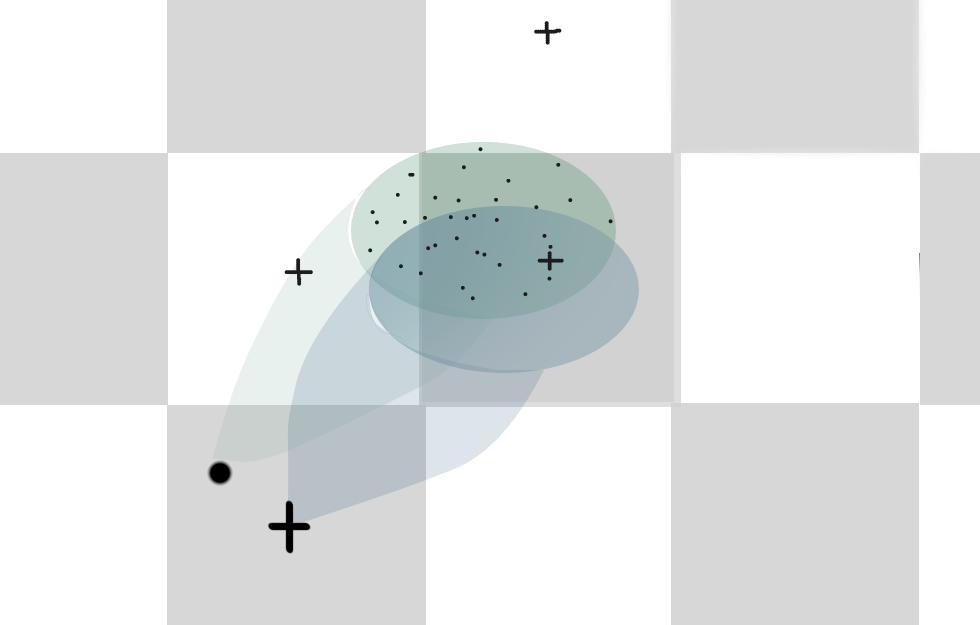
\includegraphics[width = .6\columnwidth]{figs/grid}
%	\caption{Depiction of the gridded state space. Depicted are the mean state $\hat x$ of the concrete belief MDP ($\bullet$), and the representative states $x_s$ of the abstract MDP ($\boldsymbol{+}$), together with an illustration of a stochastic transition. \textcolor{red}{should add $x_s, s, \Delta_s$, etc to figure} }
%  \label{fig:grid}
%\end{figure}

To compute $\tilde \MB\preceq^\delta_{\tilde \Labset,\Labset} \MB$, we restrict attention to simulation relations $\rel$ between states $b=(\hat x, P)$ of $\MB$ and states $\tilde x$ of $\tilde \MB $, and interfaces $\InF$, on the forms
\begin{align}
  \label{eq:rel}
    & \rel = \left\{(\tilde x, (\hat x, P ) ) \Big{|}\begin{aligned}
      (\hat x- \tilde x)^T M(\hat x-\tilde x)\leq \eps^2 \\
      P^-\preceq P \preceq   P^+
    \end{aligned} \right\}, \\
    & \InF(\tilde u,  \tilde x, \hat x)  =K( \hat x - \tilde x)+\tilde u,  \label{eq:intf}
\end{align}
for some matrices $M, P^-, P^+$ and $K$. We derive the conditions under which $\rel$ and $\InF$ define a label-based $\delta$-stochastic simulation relation between $\tilde \MB$ and $\MB$. To do so, we construct a set-valued labeling $\tilde \Labset: \Xb_{x}\rightarrow 2^\alphabeth$ and compute $\delta$ such that $\tilde \MB\preceq^\delta_{\tilde\Labset,\Labset} \MB $.

\subsubsection{Labeling requirement:}

We construct a set-valued labeling function  $\tilde \Labset: \Xb_{x}\rightarrow 2^\alphabeth$ satisfying \eqref{eq:sr-l}. For a position-based proposition $p_i$ consider, without loss of generality, a labeling $\Lab_{p_i}: \Xb\rightarrow \{\{p_i\},\emptyset\}$ for the concrete belief MDP defined by $p_i\in\Lab_p \left( (\hat x,P) \right)  \Leftrightarrow \hat x \in A$. The set-valued extension to $2^{\{\{p_i\},\emptyset\}}$ for the abstract MDP is defined as
 \begin{align}
 	\tilde \Labset_{p_i}(\tilde x) =\left\{\begin{array}{ll} \{\{p_i\}\} & \mbox{ if } \forall b \in \rel (\tilde x):p_i\in\Lab_{p_i}(b), \\
 	  \{\emptyset \} & \mbox{ if } \forall b\in \rel (\tilde x):{p_i}\not\in\Lab_{p_i}(b),\\
 	  \{\{p_i\},\emptyset\}&\mbox{ otherwise.}\end{array} \right.
 \end{align}
The labeling $\tilde \Labset_{p_i}$ can be easily computed by shrinking or expanding the set $A$ and the extension to multiple atomic propositions is straightforward. Similarly, for propositions involving the variance of the current belief state any atomic property that is monotonic\footnote{Here monotonicity of a function in $P$ is defined based on the preorder $\succeq $ for the matrices $P$ with $A\succeq B$ if $x^T(A-B)x\geq0\, \forall x\in\mathbb R^n$. } in $P$ can be mapped to the abstract model. However, atomic propositions that include probability require caution since the quantification of the probability of an event is in general not monotonic with respect to variance.


\subsubsection{Probability requirements:}
To show satisfaction of \eqref{eq:sr-2}, we need to show that there exists a $\delta$-lifting. First we require that $P^+$ (resp. $P^-$) is an upper (resp. lower) bound for $P_{k|k}$ of the belief MDP \eqref{eq:beliefx}-\eqref{eq:beliefP}.  We say that $P^-$ is a lower bound if it is a lower bound for the initial condition (see above) and   if it is monotonically increasing with respect to the Riccati equations \citep{bitmead1985monotonicity}. For the upper bound, we require, {\it mutatis mutandis}, a monotonically decreasing $P^+$.


Consider a choice of noise sources $\tilde{{s}}_{k+1}$ and $s^\Delta_{k+1}$, such that the difference between the states in \eqref{eq:abstract} and \eqref{eq:beliefx} evolves according to
\begin{equation}
\begin{aligned}
 \hat x_{k+1|k+1}-  \tilde x_{k+1}&=(A+BK)(\hat x_{k|k}-\tilde x_{k})  \\ & \qquad + P_{k+1|k}C^T s^\Delta_{k+1}+\Delta_{k+1} {\tilde{s}}_{k+1},
\end{aligned}
\end{equation}
with $\Delta_{k+1}:=(P_{k+1|k}C^T-  \tilde P C^T)$, $ \tilde{{s}}_{k+1}\sim \CA N (0,\tilde{S}_{inv})$, and $ {s}^\Delta_{k+1}\sim  \CA N (0,\  S_{k+1}^{-1}-\tilde{S}_{inv})$. 

We can now quantify the $\delta$-difference between $\MB$ and $\tilde \MB$ by verifying that for all  $(\tilde x_k,\hat x_{k|k})\in \rel$, with probability at least $1-\delta$ it holds that $(\tilde x_{k+1},\hat x_{k+1|k+1})\in \rel$. %\axx{The first entry in last two pairs should be tilde?}
% thnx
%Furthermore, for all $\hat x_{k+1}$, there exists $x_\grid \in \ball_\grid (0)$ such that  $\hat x_{k+1}+x_\grid = x_s$ for some $s \in \mathbb{S}$. Therefore we can write the update of the difference expression in \eqref{eq:rel} as
%\begin{equation}
%\begin{aligned}
% \hat x_{k+1|k+1} - x_{s_{k+1}}=(A+BK)(\hat x_{k|k}- x_{s,k})+x_\grid \\ + \bar P   C^T s^\Delta_{k+1} +\Delta_{k+1}( \hat{\red{s}}_{k+1}+ \red{s}^\Delta_{k+1}).
%\end{aligned}
%\end{equation}
Furthermore, we can bound the norm of the noise terms ${s}^\Delta_{k+1}$ and $ \tilde{{s}}_{k+1}$ using probabilistic guarantees computed via inter alia the chi-square distribution. The computation of the values of $\epsilon$ and the values of the matrices  in $\rel$ \eqref{eq:rel} and in the interface \eqref{eq:intf}, can now be performed via sequential convex optimizations expressed with linear matrix inequalities \citep{haesaert2017verification}.

\begin{remark}
  Here we did not explicitly write out the lifted probability space $\mathbb{W}_t$ of Definition \ref{def:kernellift}. It is obtained from the probability measure induced by joint evolution of \eqref{eq:beliefx} and \eqref{eq:abstract} driven by noise sources $s^\Delta$ and $ {\tilde{s}} $.
 \end{remark}

\subsubsection{Initial condition requirement:} For the satisfaction of \eqref{eq:sr-1}, we repeat the same procedure as above and show that there exists an initial state $\tilde x_{0}$ (or if needed a distribution) for $\tilde \MB$ such that $\tilde x_{0} \bar\rel_\delta \initb$.

Combined, these requirements constitute sufficient conditions for Theorem \ref{thm:main} to apply for a Kalman belief model $\MB$ and an abstraction $\tilde \MB$ on the form \eqref{eq:abstract}. As mentioned above, a grid-based abstraction can then be constructed from $\tilde \MB$ to obtain a finite abstraction $\tilde \MB_{grid}$ such that $\tilde \MB_{grid} \preceq^{\delta_{grid}}_{\tilde \Labset_{grid},\tilde \Labset} \tilde \MB \preceq^\delta_{\tilde \Labset,\Labset} \MB$. While $\MB$ is of dimension $n + n^2$, $\tilde \MB$ is of dimension $n$, therefore this intermediate step is crucial to mitigate the curse of dimensionality in the gridding procedure.

\begin{figure}[h]
	\centering
	
\includegraphics[width=0.7\columnwidth]{figs/rover.jpg}
	\caption{NASA JPL Mars rover.}
	\label{fig:rover}
\end{figure}

%%%%%%%%%%%%%%%%%%%%%%%%%%%%%%%

\section{Case study}\label{sec:case}

Motivated by autonomy in space exploration applications, we consider a rover (Fig. \ref{fig:rover}) tasked with identifying and collecting scientific samples in a partially unknown Mars environment. In this scenario, there exist a very low-resolution map of the Mars surface (i.e., environment) from satellite imagery. While different region types can be identified on the surface from this overhead imagery, the accuracy of labelling is not sufficient for near-surface operations. Here we consider two types of regions: \emph{target regions} and \emph{risk regions}, where the former are expected to contain science samples and the latter may contain non-traversable areas such as obstacles, steep slopes, loose sand, etc.

\textbf{Rover model.} We consider a simple rover modeled as a point mass $x_k \in \mathbb{R}^2$ affected by stochastic disturbances. In a real-world setting the position of the rover cannot be measured perfectly, so we model its dynamics as a partially-observable system:
\begin{equation*}
\begin{aligned}
  x_{k+1}&= x_{k} + u_k+ w_k,  & w_k \sim \CA N \left(0,\begin{bsmallmatrix}.4&-.2\\-.2&.4\end{bsmallmatrix}\right),  \\
  z_k&= x_k+v_k,  & v_k \sim \CA N \left(0,\begin{bsmallmatrix}1&0\\0&1\end{bsmallmatrix}\right). \phantom{1234} \hspace{0.6mm}
\end{aligned}
\end{equation*}
The corresponding belief space model $\MB$ is defined by the Kalman filter equations \eqref{eq:beliefx}-\eqref{eq:beliefP} as in Section \ref{sec:gaussian}. We assume that at the initial time instance, the belief distribution of $x$ is $\mathcal N(\hat x_0, P_0)$ with $P_0=\begin{bsmallmatrix} 
 0.74446& -0.2862\\
 -0.2862 &  0.74446
\end{bsmallmatrix}. 
 $


\textbf{Environment model.} From the overhead imagery, we consider two %potential
 target regions $T_1$ and $T_2$ where the probability of encountering a desired sample has been assessed as 0.5 and 0.6, respectively. In addition, there are two risk regions $R_1$ and $R_2$ with probabilities of 0.9 and 0.7 that the rover can traverse them safely, respectively. For both target and risk regions, we assume that the true nature of the region can be determined via measurements from on-board sensors when the rover is within a certain distance of the regions. The regions are illustrated in Fig. \ref{fig:exp1}, along with the regions from where measurements can be acquired (dashed lines). To each region we associate a discrete belief state $b_r \in \{ p_{r,0}, 1, 0 \}$ where $p_{r,0}$ are the belief probabilities from satellite imagery, with dynamics illustrated in Fig. \ref{fig:envmdp}.

\begin{figure}[t]
  \begin{center}
  \begin{tikzpicture}
    \node[draw, minimum width=0.75cm, node distance=2.5cm, circle, initial above,initial text={} ] (b0) {$p_0$};
    \node[draw, minimum width=0.75cm, node distance=2.5cm, circle, right of=b0] (b1) {0};
    \node[draw, minimum width=0.75cm, node distance=2.5cm, circle, right of=b1] (b2) {1};

    \draw[-latex, red] (b0) to node[black, above] {$p = 1-p_0$} (b1);
    \draw[-latex, red] (b0) to[out=45, in=145] node[black, above] {$p = p_0$} (b2);

    \draw[-latex, blue, dashed] (b0) to[loop left] (b0);
    \draw[-latex, red] (b1) to[loop right] (b1);
    \draw[-latex, red] (b2) to[loop right] (b2);
    \draw[-latex, blue, dashed] (b1) to[loop above] (b1);
    \draw[-latex, blue, dashed] (b2) to[loop above] (b2);
  \end{tikzpicture}
  \end{center}
  \caption{Illustration of environment belief model for a single region. At the beginning the belief is $p_0$. When a measurement is received (solid red edges), the belief transitions to $1$ with probability $p_0$ and to $0$ with probability $1-p_0$. That is, one measurement is sufficient to determine the state of the region. When no measurement is taken (blue dashed edges), or if a measurement has already been taken, the state does not change.}
  \label{fig:envmdp}
\end{figure}


\begin{figure}[b]
  \footnotesize
  % This file was created by matplotlib2tikz v0.6.14.
\centering
\begin{tikzpicture}
\newlength\figurewidth
\newlength\figureheight
\setlength\figurewidth{\columnwidth}
\setlength\figureheight{.4\columnwidth}
\definecolor{color0}{rgb}{0.12156862745098,0.466666666666667,0.705882352941177}

\begin{axis}[scale =.8,
xlabel={$\delta$},
ylabel={$\epsilon$},
xmin=-0.01395, xmax=0.25,
ymin=0.8, ymax=1.45222764450879,
width=\figurewidth,
height=\figureheight,
% tick align=outside,
% tick pos=left,
x grid style={lightgray!92.026143790849673!black},
y grid style={lightgray!92.026143790849673!black},
axis y line=left,
axis x line=middle,
every axis x label/.style={
    at={(ticklabel* cs:1.05)}
}
]
\addplot [semithick, color0, forget plot,  mark=*,mark options={scale=.84}]
table {%
0.001 1.4272384844875
0.0167368421052632 1.22339465219428
0.0324736842105263 1.16617411196529
0.0482105263157895 1.13191279574885
0.0639473684210526 1.10601589042324
0.0796842105263158 1.08400668945514
0.0954210526315789 1.06721503359466
0.111157894736842 1.05265893349788
0.126894736842105 1.04157018327801
0.142631578947368 1.02417176675944
0.158368421052632 1.01254639660019
0.174105263157895 1.00120158889137
0.189842105263158 0.991557539021032
0.205578947368421 0.982277989301703
0.221315789473684 0.97353496742902
0.237052631578947 0.965239656823681
0.252789473684211 0.960158902624749
0.268526315789474 0.951512372393061
0.284263157894737 0.927455284061691
0.3 0.935781247731614
};
\end{axis}

\end{tikzpicture}
  \caption{Trade-off between state error $\epsilon$ from Eq. \eqref{eq:rel} and probability error $\delta$ from Definition \ref{def:apbsim}.}
  \label{fig:tradeoff}
\end{figure}

With $\MB_{env}$ as the combined environment model with state $(b_{T_1}, b_{T_2}, b_{R_1}, b_{R_2})$, the overall system is $\MB \otimes \MB_{env}$. This product is defined similarly to the product in Definition \ref{def:product}: $\MB$ gives inputs to $\MB_{env}$ according to the position in the state space. If the state estimate $\hat x$ of $\MB$ is inside a measurement region (dashed lines in Fig. \ref{fig:exp1}), a measurement is performed in the corresponding environment MDP (red edge in Fig. \ref{fig:envmdp}).


\textbf{Specification.} The objective is to collect a sample while avoiding unsafe regions. To this end, we consider the scLTL specification
\begin{equation}
  \psi =\lnot \texttt{fail} \; \mathcal {U} \; \texttt{sample},
\end{equation}
where the atomic proposition \texttt{sample} is true if the rover is in a target region that contains a sample, and the atomic proposition \texttt{fail} is defined as being true if the rover is in a risk region that contains an obstacle.


\textbf{Solution.} We first construct a finite abstraction of $\MB$ as outlined in the previous section; first we compute an approximate LTI belief model and then we  discretize the state space $[-10, 10]^2$ with  grids of size $\grid = (0.76481, 0.64426)$. The input space $[-1,1]^2$ is sampled with nine discrete inputs $\{0, 1, -1\}^2$. Fig.  \ref{fig:tradeoff} illustrates the trade-off between the $\epsilon$ error in the relation \eqref{eq:rel} and the $\delta$-difference in Definition \ref{def:apbsim} for these choices of discretization parameters. Combined with a relaxation of the labeling as introduced in the previous subsection, %and introducing a simulation relation that compensates for accuracy loss caused by the gridding, 
we obtain an abstract model $\tilde \MB_{grid}$ with the property that $\tilde \MB_{grid}\preceq^{0.01}_{\tilde\Labset_{grid},\Labset} \MB $. Remark that the upper bound $P^+$ and the lower bound $P^- $ have been selected based on the steady state Kalman gain, and based on the initial covariance $P_0$, respectively.

In order to analyze the combined system $\MB \otimes \MB_{env}$, we create $\tilde \MB_{grid} \otimes \MB_{env}$ as a nondeterministic product and treat it analogously to the nondeterminism in the connection between an MDP and a DFSA in Eq. \eqref{eq:prob:robust_optimal}. Effectively, when there is uncertainty about whether a measurement of a region can be expected, the worst-case is considered in the value iteration which by Theorem \ref{thm:main} ensures that the obtained probabilities are indeed lower bounds. 

With this method we compute a value function and an associated control policy for $\tilde \MB_{grid} \otimes \MB_{env}$ and refine it to the concrete system. The resulting policy takes inputs from $\Xb \times \prod_{i=1}^4 \{ p_{0,i}, 0, 1 \}$---the combined rover and environment state---and has internal memory dynamics given by the specification DFSA. The value function is illustrated in Fig. \ref{fig:valuefcn} for two different environment states.

\begin{figure}
  \footnotesize
  \begin{tikzpicture}
    \begin{axis}[
      name=ax1,
      at = {(0,0)},
      width=0.55\columnwidth,
      height=0.55\columnwidth,
      anchor = south west,
      xmin=-10,
      xmax=10,
      ymin=-10,
      ymax=10,
      ticks=none]
      \addplot graphics[xmin=-10,ymin=-10,xmax=10,ymax=10] {figs/value1.pdf};
    \end{axis}
    \begin{axis}[
      name=ax2,
      at = {(0.4\columnwidth,0)},
      width=0.55\columnwidth,
      height=0.55\columnwidth,
      anchor = south west,
      xmin=-10,
      xmax=10,
      ymin=-10,
      ymax=10,
      ticks=none]
      \addplot graphics[xmin=-10,ymin=-10,xmax=10,ymax=10] {figs/value2.pdf};
    \end{axis}
    \node[anchor=south west] (cbar) at (0.8\columnwidth,-1.1mm) {
\includegraphics[width=0.03\columnwidth, height=0.372\columnwidth]{figs/cbar.pdf}};
    \node[anchor=west, yshift=2mm] at (cbar.south east) {$V = 0$};
    \node[anchor=west, yshift=-2mm] at (cbar.north east) {$V = 1$};
    \node[anchor=west, ] at (cbar.east) {$V = 0.5$};
  \end{tikzpicture}
  \caption{Illustration of value function for two different states of the environment, with regions of interest plotted with dashed lines. Left: environment state $(0.5, 0.6, 0.9, 0.7)$, i.e., all regions are still uncertain, which results in a fairly uniform value function with slightly less success probability close to the risk regions. Right: environment state $(0.5, 1, 0.9, 0)$, i.e., it is known that $T_2$ contains a sample and that $R_2$ contains an obstacle, which yields a more polarized value function.}
  \label{fig:valuefcn}
\end{figure}

\begin{figure}
  \footnotesize
  \setlength\figurewidth{0.65\columnwidth}
  \setlength\figureheight{0.6\columnwidth}

  \begin{center}
    % This file was created by matplotlib2tikz v0.6.14.
\begin{tikzpicture}

\definecolor{color1}{rgb}{1,0.498039215686275,0.0549019607843137}
\definecolor{color0}{rgb}{0.12156862745098,0.466666666666667,0.705882352941177}
\definecolor{color3}{rgb}{0.83921568627451,0.152941176470588,0.156862745098039}
\definecolor{color2}{rgb}{0.172549019607843,0.627450980392157,0.172549019607843}
\definecolor{color5}{rgb}{0.549019607843137,0.337254901960784,0.294117647058824}
\definecolor{color4}{rgb}{0.580392156862745,0.403921568627451,0.741176470588235}

\begin{axis}[
xlabel={$x_1$},
ylabel={$x_2$},
xmin=-11.1088588047251, xmax=11.1145664581499,
ymin=-10.1108621762447, ymax=10.9576601036307,
width=\figurewidth,
height=\figureheight,
tick align=outside,
tick pos=left,
mark size=1,
x grid style={lightgray!92.026143790849673!black},
y grid style={lightgray!92.026143790849673!black}
]
\addplot [only marks, draw=black, fill=black, colormap/viridis]
table{%
x                      y
-1.000000000000000e+01 -9.000000000000000e+00
-8.869595294321220e+00 -7.814207719224903e+00
-7.104778400743559e+00 -7.140354399223419e+00
-6.376752541526766e+00 -6.870554896721502e+00
-4.832702844468539e+00 -6.036032413666041e+00
-4.377547654253716e+00 -5.216915548266608e+00
-3.744230908366174e+00 -3.905880113729608e+00
-2.871984978581734e+00 -2.567990703687725e+00
-3.127375571989979e+00 -2.090610019084363e+00
-2.305771899885637e+00 -9.338180566109633e-01
-3.687373068419801e+00 +4.769618066414293e-01
-4.131753222593663e+00 +9.557682476343059e-01
-4.601633165510158e+00 +1.661042239367786e+00
-5.694730614871723e+00 +4.003513878529873e+00
-5.973575212285128e+00 +3.578554273124150e+00
-6.299886148045688e+00 +3.044114991420233e+00
-4.771656903671562e+00 +2.858962077904698e+00
-4.543639365229525e+00 +2.139567825321754e+00
-2.673138926724003e+00 +1.798961623791945e+00
-3.527414786094551e+00 +3.231833707854521e+00
-2.124252800165384e+00 +2.332430078604584e+00
-1.336517727306551e+00 +1.867196593378676e+00
-1.601443252054275e+00 +2.126202270702624e+00
-2.276211315148957e+00 +3.308254449757351e+00
-7.301645225187249e-01 +4.522420844572547e+00
+6.421309072702257e-01 +5.679192620151055e+00
+6.291550303486995e-01 +6.527896371328548e+00
+1.619950872445812e+00 +7.559823424104585e+00
+3.103218944956174e+00 +6.190024650395538e+00
+5.076329139729479e+00 +6.568676876712611e+00
+5.892120984615905e+00 +7.942903477538653e+00
+5.647060738990990e+00 +8.410805253485940e+00
+6.378542919870930e+00 +7.216198212323969e+00
+5.911651447016797e+00 +6.074808626739333e+00
};
\addplot [only marks, draw=black, fill=black, colormap/viridis]
table{%
x                      y
-6.000000000000000e+00 -9.000000000000000e+00
-5.901406929599968e+00 -7.508199438071110e+00
-4.358884763233826e+00 -5.792082591551480e+00
-3.919800671528496e+00 -4.077694923566842e+00
-3.692867013779527e+00 -2.339134536400095e+00
-4.122397810293728e+00 -8.975301878708711e-01
-2.490405176513862e+00 -2.573953379208296e-01
-4.111781121286302e+00 +1.145086563115543e+00
-3.677892980298973e+00 +1.377137896197289e+00
-3.566602837148350e+00 +8.815148406364688e-01
-3.338101562637621e+00 +1.932094838504950e+00
-4.516623627187172e+00 +2.134782889471700e+00
-5.049009747014780e+00 +3.556356142323278e+00
-5.015975542724512e+00 +4.642632272866249e+00
-4.249031141395299e+00 +3.638868112650753e+00
-3.606475659338956e+00 +3.327243509372837e+00
-2.389126541991601e+00 +2.001450651124150e+00
-1.783057348634495e+00 +1.573015875488078e+00
-2.981625704030834e+00 +3.183156711833124e+00
-2.358357517805116e+00 +4.479839517723944e+00
-2.288659157327666e+00 +6.279107959374064e+00
-1.411436975902111e+00 +6.189266978612975e+00
-5.320073996643725e-01 +6.157716555765220e+00
-5.104133024329928e-01 +7.405451568002405e+00
+1.274177610274697e+00 +5.346446814476317e+00
+3.328125868896929e+00 +5.848995543358567e+00
+3.432597856511344e+00 +7.459258972502006e+00
+4.030094855910188e+00 +7.728847292266309e+00
+5.354424702892910e+00 +8.500182463536220e+00
+6.155873129399546e+00 +6.918829831869020e+00
+5.925808542673061e+00 +6.475595415762200e+00
};
\addplot [only marks, draw=black, fill=black, colormap/viridis]
table{%
x                      y
-2.000000000000000e+00 -9.000000000000000e+00
-3.044462714452268e+00 -7.306350162100894e+00
-2.293090798054657e+00 -7.301138964922043e+00
-2.992445270727864e+00 -5.860237642906498e+00
-2.700570628355699e+00 -5.891003937213707e+00
-3.261421640643176e+00 -4.215783895557847e+00
-3.158411977295807e+00 -2.780961678014854e+00
-3.143450533987836e+00 -2.507508068387384e+00
-3.025567040118594e+00 -2.323985887674691e+00
-3.147878570292180e+00 -1.765176888234320e+00
-3.321097798094850e+00 -8.960733607114131e-01
-3.071809481398453e+00 +2.656018153234110e-01
-3.347289674472285e+00 +2.525143550310250e+00
-4.343077763169791e+00 +3.655246402097009e+00
-4.746507006214285e+00 +4.694914521302897e+00
-4.773216787388434e+00 +4.346197557892083e+00
-4.295952786822955e+00 +3.660497376626418e+00
-3.143953286965482e+00 +2.625049791199087e+00
-1.641162836868084e+00 +2.688373056222609e+00
-2.041754565063155e+00 +2.649157162515526e+00
-3.306752490703531e+00 +3.253350556635815e+00
-2.983336851770111e+00 +3.971825313172622e+00
-2.469010596282821e+00 +4.546595568617136e+00
-1.228788797359903e+00 +5.627707538998200e+00
-1.094952620493618e+00 +8.175427155795038e+00
-9.592574172669480e-01 +8.082721342294306e+00
-1.194386354456936e+00 +8.165264896530068e+00
-4.616822792871155e-01 +6.621700444105216e+00
+7.497631277014686e-01 +7.076610441120152e+00
+1.979746828542337e+00 +6.612237335050672e+00
+3.128826364302311e+00 +6.253528797214032e+00
+4.025272616622998e+00 +6.503242452969750e+00
+3.645362150228443e+00 +7.636106778389254e+00
+5.261846571766094e+00 +6.237023538647955e+00
+5.641826018152110e+00 +7.725113353647728e+00
+6.812612257678752e+00 +7.585618827435113e+00
+6.232989074320007e+00 +8.719742643797003e+00
};
\addplot [only marks, draw=black, fill=black, colormap/viridis]
table{%
x                      y
+2.000000000000000e+00 -9.000000000000000e+00
+2.952866870372958e+00 -8.576100227432466e+00
+4.242197553383458e+00 -7.804545716747594e+00
+5.074855341092752e+00 -5.625352120055734e+00
+4.830608053317017e+00 -5.307135825638624e+00
+6.260668707794887e+00 -4.393024727214535e+00
+5.626132234535231e+00 -3.468882934108938e+00
+4.360920432033688e+00 -1.633814410374898e+00
+5.283892683157318e+00 -9.239872896419613e-01
+6.137055506057617e+00 -2.713402990434055e-01
+3.960819582615776e+00 +7.198393840378496e-01
+4.348495153676051e+00 +2.182925104805387e+00
+5.310490549051644e+00 +3.346073054040058e+00
+5.927805236978374e+00 +3.532146335797724e+00
+7.076206486765265e+00 +4.595056538443954e+00
+6.905541839334503e+00 +6.818868569963236e+00
+6.916859672204205e+00 +6.538704789396275e+00
};
\addplot [only marks, draw=black, fill=black, colormap/viridis]
table{%
x                      y
+6.000000000000000e+00 -9.000000000000000e+00
+7.656026307682226e+00 -7.552110273740422e+00
+6.106733751763857e+00 -4.944778792524008e+00
+5.007607308637190e+00 -4.476890270578113e+00
+5.340307715623565e+00 -3.870524755975019e+00
+5.223674090042989e+00 -2.999138613814250e+00
+4.852825372926093e+00 -1.649771429171313e+00
+5.277460910519775e+00 -6.637444320456167e-01
+3.912214555867033e+00 +4.809921810937652e-01
+4.689101241974543e+00 +1.514074549520304e+00
+5.988818016236550e+00 +1.998528533661037e+00
+5.506348480377154e+00 +3.663415125077347e+00
+5.339192804183695e+00 +4.558762439747721e+00
+7.256112587009863e+00 +5.131362769874022e+00
+7.631959808780144e+00 +5.683576842740282e+00
+7.257947121647226e+00 +7.090711607035485e+00
+6.414874444391497e+00 +6.824546651611620e+00
};
\addplot [only marks, draw=black, fill=black, colormap/viridis]
table{%
x                      y
+1.000000000000000e+01 -9.000000000000000e+00
+8.501744459872617e+00 -7.514163496353530e+00
+7.502543301317530e+00 -6.247529485824156e+00
+6.789481505237688e+00 -5.327060783448672e+00
+6.299648866376312e+00 -4.120122662433571e+00
+4.477615169608585e+00 -3.392450768338643e+00
+5.941939396771113e+00 -2.155271399521218e+00
+4.924919113275441e+00 -1.405474597240854e+00
+4.038299633666932e+00 -2.035680327253797e-01
+5.189304536388701e+00 +1.018679026545901e+00
+4.395910542655945e+00 +2.158524989021073e+00
+6.551109435674287e+00 +2.948566939226978e+00
+6.949044679173154e+00 +3.493783802114474e+00
+4.470283883624948e+00 +5.678295462897534e+00
+7.557669000755279e+00 +6.353439694488499e+00
+7.116516078033896e+00 +6.021511860498869e+00
};
\path [draw=red, fill=red, opacity=0.5] (axis cs:2,-5)
--(axis cs:2,2)
--(axis cs:0,2)
--(axis cs:0,-5)
--cycle;

\path [draw=red, fill=red, opacity=0.5] (axis cs:2,3)
--(axis cs:2,10)
--(axis cs:0,10)
--(axis cs:0,3)
--cycle;

\path [draw=blue, fill=blue, opacity=0.5] (axis cs:-6,6)
--(axis cs:-6,9)
--(axis cs:-9,9)
--(axis cs:-9,6)
--cycle;

\path [draw=blue, fill=blue, opacity=0.5] (axis cs:9,6)
--(axis cs:9,9)
--(axis cs:6,9)
--(axis cs:6,6)
--cycle;

\addplot [semithick, color0, forget plot]
table {%
-10 -9
-8.86959529432122 -7.8142077192249
-7.10477840074356 -7.14035439922342
-6.37675254152677 -6.8705548967215
-4.83270284446854 -6.03603241366604
-4.37754765425372 -5.21691554826661
-3.74423090836617 -3.90588011372961
-2.87198497858173 -2.56799070368773
-3.12737557198998 -2.09061001908436
-2.30577189988564 -0.933818056610963
-3.6873730684198 0.476961806641429
-4.13175322259366 0.955768247634306
-4.60163316551016 1.66104223936779
-5.69473061487172 4.00351387852987
-5.97357521228513 3.57855427312415
-6.29988614804569 3.04411499142023
-4.77165690367156 2.8589620779047
-4.54363936522953 2.13956782532175
-2.673138926724 1.79896162379194
-3.52741478609455 3.23183370785452
-2.12425280016538 2.33243007860458
-1.33651772730655 1.86719659337868
-1.60144325205428 2.12620227070262
-2.27621131514896 3.30825444975735
-0.730164522518725 4.52242084457255
0.642130907270226 5.67919262015106
0.629155030348699 6.52789637132855
1.61995087244581 7.55982342410458
3.10321894495617 6.19002465039554
5.07632913972948 6.56867687671261
5.8921209846159 7.94290347753865
5.64706073899099 8.41080525348594
6.37854291987093 7.21619821232397
5.9116514470168 6.07480862673933
};
\addplot [semithick, color1, forget plot]
table {%
-6 -9
-5.90140692959997 -7.50819943807111
-4.35888476323383 -5.79208259155148
-3.9198006715285 -4.07769492356684
-3.69286701377953 -2.3391345364001
-4.12239781029373 -0.897530187870871
-2.49040517651386 -0.25739533792083
-4.1117811212863 1.14508656311554
-3.67789298029897 1.37713789619729
-3.56660283714835 0.881514840636469
-3.33810156263762 1.93209483850495
-4.51662362718717 2.1347828894717
-5.04900974701478 3.55635614232328
-5.01597554272451 4.64263227286625
-4.2490311413953 3.63886811265075
-3.60647565933896 3.32724350937284
-2.3891265419916 2.00145065112415
-1.7830573486345 1.57301587548808
-2.98162570403083 3.18315671183312
-2.35835751780512 4.47983951772394
-2.28865915732767 6.27910795937406
-1.41143697590211 6.18926697861298
-0.532007399664372 6.15771655576522
-0.510413302432993 7.40545156800241
1.2741776102747 5.34644681447632
3.32812586889693 5.84899554335857
3.43259785651134 7.45925897250201
4.03009485591019 7.72884729226631
5.35442470289291 8.50018246353622
6.15587312939955 6.91882983186902
5.92580854267306 6.4755954157622
};
\addplot [semithick, color2, forget plot]
table {%
-2 -9
-3.04446271445227 -7.30635016210089
-2.29309079805466 -7.30113896492204
-2.99244527072786 -5.8602376429065
-2.7005706283557 -5.89100393721371
-3.26142164064318 -4.21578389555785
-3.15841197729581 -2.78096167801485
-3.14345053398784 -2.50750806838738
-3.02556704011859 -2.32398588767469
-3.14787857029218 -1.76517688823432
-3.32109779809485 -0.896073360711413
-3.07180948139845 0.265601815323411
-3.34728967447229 2.52514355031025
-4.34307776316979 3.65524640209701
-4.74650700621429 4.6949145213029
-4.77321678738843 4.34619755789208
-4.29595278682296 3.66049737662642
-3.14395328696548 2.62504979119909
-1.64116283686808 2.68837305622261
-2.04175456506316 2.64915716251553
-3.30675249070353 3.25335055663581
-2.98333685177011 3.97182531317262
-2.46901059628282 4.54659556861714
-1.2287887973599 5.6277075389982
-1.09495262049362 8.17542715579504
-0.959257417266948 8.08272134229431
-1.19438635445694 8.16526489653007
-0.461682279287116 6.62170044410522
0.749763127701469 7.07661044112015
1.97974682854234 6.61223733505067
3.12882636430231 6.25352879721403
4.025272616623 6.50324245296975
3.64536215022844 7.63610677838925
5.26184657176609 6.23702353864796
5.64182601815211 7.72511335364773
6.81261225767875 7.58561882743511
6.23298907432001 8.719742643797
};
\addplot [semithick, color3, forget plot]
table {%
2 -9
2.95286687037296 -8.57610022743247
4.24219755338346 -7.80454571674759
5.07485534109275 -5.62535212005573
4.83060805331702 -5.30713582563862
6.26066870779489 -4.39302472721454
5.62613223453523 -3.46888293410894
4.36092043203369 -1.6338144103749
5.28389268315732 -0.923987289641961
6.13705550605762 -0.271340299043406
3.96081958261578 0.71983938403785
4.34849515367605 2.18292510480539
5.31049054905164 3.34607305404006
5.92780523697837 3.53214633579772
7.07620648676526 4.59505653844395
6.9055418393345 6.81886856996324
6.9168596722042 6.53870478939627
};
\addplot [semithick, color4, forget plot]
table {%
6 -9
7.65602630768223 -7.55211027374042
6.10673375176386 -4.94477879252401
5.00760730863719 -4.47689027057811
5.34030771562356 -3.87052475597502
5.22367409004299 -2.99913861381425
4.85282537292609 -1.64977142917131
5.27746091051977 -0.663744432045617
3.91221455586703 0.480992181093765
4.68910124197454 1.5140745495203
5.98881801623655 1.99852853366104
5.50634848037715 3.66341512507735
5.3391928041837 4.55876243974772
7.25611258700986 5.13136276987402
7.63195980878014 5.68357684274028
7.25794712164723 7.09071160703548
6.4148744443915 6.82454665161162
};
\addplot [semithick, color5, forget plot]
table {%
10 -9
8.50174445987262 -7.51416349635353
7.50254330131753 -6.24752948582416
6.78948150523769 -5.32706078344867
6.29964886637631 -4.12012266243357
4.47761516960859 -3.39245076833864
5.94193939677111 -2.15527139952122
4.92491911327544 -1.40547459724085
4.03829963366693 -0.20356803272538
5.1893045363887 1.0186790265459
4.39591054265594 2.15852498902107
6.55110943567429 2.94856693922698
6.94904467917315 3.49378380211447
4.47028388362495 5.67829546289753
7.55766900075528 6.3534396944885
7.1165160780339 6.02151186049887
};
\node at (axis cs:1,1)[
  scale=0.5,
  anchor=base west,
  text=black,
  rotate=0.0
]{ $O_1$};
\node at (axis cs:1,9)[
  scale=0.5,
  anchor=base west,
  text=black,
  rotate=0.0
]{ $O_2$};
\node at (axis cs:-9,8)[
  scale=0.5,
  anchor=base west,
  text=black,
  rotate=0.0
]{ $T_1$};
\node at (axis cs:8,8)[
  scale=0.5,
  anchor=base west,
  text=black,
  rotate=0.0
]{ $T_2$};
\end{axis}

\end{tikzpicture}   % This file was created by matplotlib2tikz v0.6.14.
\begin{tikzpicture}

\definecolor{color1}{rgb}{1,0.498039215686275,0.0549019607843137}
\definecolor{color0}{rgb}{0.12156862745098,0.466666666666667,0.705882352941177}
\definecolor{color2}{rgb}{0.172549019607843,0.627450980392157,0.172549019607843}

\begin{axis}[
mark size = 0.5,
ticks=none,
xmin=-11, xmax=11,
ymin=-10.6290882408405, ymax=10.9823375352781,
width=\figurewidth,
height=\figureheight,
tick align=outside,
tick pos=left,
x grid style={lightgray!92.026143790849673!black},
y grid style={lightgray!92.026143790849673!black}
]
\addplot [only marks, draw=black, fill=black, colormap/viridis]
table{%
x                      y
-8.000000000000000e+00 -9.000000000000000e+00
-8.281791193811282e+00 -6.953277059756937e+00
-6.609947231673338e+00 -7.304755895777043e+00
-6.447420151999264e+00 -6.984253859219061e+00
-5.930025319876885e+00 -6.296279125763103e+00
-5.476123458484502e+00 -6.049868453584115e+00
-4.680375628377898e+00 -4.982516422756326e+00
-3.356608221836718e+00 -4.767445283086258e+00
-3.850337386959414e+00 -3.882953851781119e+00
-3.888519145722516e+00 -3.480146659512000e+00
-5.320305970691908e+00 -2.277119535242806e+00
-4.379722627893722e+00 -3.023297381626749e+00
-2.966831046751209e+00 -2.008805754832921e+00
-4.696058526749306e+00 +1.019091306738935e-01
-4.628219306657023e+00 +1.300100090541606e+00
-5.641564937919985e+00 +1.796635145522380e+00
-6.307184225641461e+00 +2.288130625455808e+00
-7.217828733789983e+00 +3.143921812081298e+00
-7.301911031188013e+00 +4.255956608402649e+00
-6.401344954223192e+00 +5.270680166902547e+00
-8.171856419882948e+00 +6.563080734161627e+00
};
\addplot [only marks, draw=black, fill=black, colormap/viridis]
table{%
x                      y
+0.000000000000000e+00 -9.000000000000000e+00
+2.985780663708160e-02 -8.155463278156050e+00
+1.071409254737555e+00 -8.202590105544974e+00
+2.130577217930679e+00 -8.147034783291767e+00
+3.046653997506764e+00 -7.814782310273142e+00
+2.993503950729483e+00 -6.732513426782055e+00
+3.364980364937721e+00 -5.919601911047740e+00
+4.577267269183741e+00 -5.442531058948178e+00
+4.641924364448064e+00 -4.277469389688367e+00
+4.066522550812240e+00 -2.261074508296681e+00
+4.900884132823337e+00 -1.747839224197387e+00
+5.242948546817824e+00 -1.658932790996334e+00
+4.951650027020797e+00 -5.458682191996835e-01
+5.160727075484108e+00 +1.786499818804027e-02
+4.951600531141041e+00 +3.796585040088380e-01
+5.548111410812709e+00 +9.093914656273301e-01
+5.998289710281483e+00 +1.845859092339620e+00
+5.586468819814069e+00 +2.958893844938457e+00
+6.773322394657046e+00 +4.341573264475908e+00
+6.244801362810740e+00 +3.255339248138667e+00
+5.386058184710604e+00 +2.832977405694789e+00
+3.382447161292124e+00 +5.131303079674516e+00
+4.874337596806267e+00 +2.495954941054408e+00
+4.650503806334480e+00 +3.995285095184848e-01
+5.025471920274055e+00 -5.406637729947061e-01
+3.653106795537211e+00 -2.331886810567701e+00
+3.777550916600270e+00 -3.262576207290882e+00
+4.208193801414156e+00 -5.223790221008551e+00
+4.894433739744199e+00 -6.435884403595750e+00
+3.799772582533073e+00 -8.195765033159091e+00
+1.063593830208735e+00 -7.803367444083015e+00
-1.186440212491861e+00 -8.416040749834128e+00
-1.769357566346293e+00 -8.393133290175719e+00
-3.454943820617372e+00 -7.829608609619289e+00
-4.718419194171268e+00 -6.806453261226547e+00
-7.128929570346833e+00 -5.582933784317277e+00
-6.754145560982441e+00 -4.927567852678047e+00
-7.809944106601641e+00 -3.287103405394836e+00
-7.608490106653687e+00 -2.786103027237490e+00
-6.664925925528791e+00 -2.687368525725410e+00
-6.819564565858922e+00 -2.207441188034236e+00
-6.119656171566637e+00 -2.321958612214557e+00
-5.398012336881704e+00 -6.633452969104143e-01
-6.326849807413460e+00 +6.558845980278348e-01
-6.175272895510815e+00 +1.444858418003883e+00
-7.632034853475458e+00 +3.355390912891568e+00
-6.251375019139898e+00 +4.004939418758159e+00
-6.160033028437569e+00 +4.084610663102694e+00
-5.910891233600980e+00 +3.553568231521559e+00
-7.187232311111987e+00 +4.703244684591716e+00
-8.802150302563509e+00 +8.035950400947264e+00
};
\addplot [only marks, draw=black, fill=black, colormap/viridis]
table{%
x                      y
+8.000000000000000e+00 -9.000000000000000e+00
+8.511205582201939e+00 -9.490847881526234e+00
+8.123691607827535e+00 -8.945490678745058e+00
+8.263822914662137e+00 -7.614276297182030e+00
+7.514100738376864e+00 -8.134440925432358e+00
+7.298345618417102e+00 -7.124767904275431e+00
+5.661620747278767e+00 -6.163981262845379e+00
+4.308129478899167e+00 -4.248895613551244e+00
+4.661943867045995e+00 -3.734081630931301e+00
+6.045638341595694e+00 -3.283722422053446e+00
+4.311200610860274e+00 -3.054620213961065e+00
+3.764155218303413e+00 -1.339286613286621e+00
+4.507407456386630e+00 -6.260285666477190e-01
+6.195941762467750e+00 -1.751868652546797e+00
+5.652298276850433e+00 -1.433432909888064e+00
+6.004475142579373e+00 -1.176455188056848e+00
+7.867024860002735e+00 -1.436677206342497e+00
+6.149524945185612e+00 -1.765396180120760e-02
+7.231136140072594e+00 -2.834317843654784e-01
+5.357245998891423e+00 +1.116871382840182e+00
+4.924762093179862e+00 +2.175740570857628e+00
+6.145247254490910e+00 +1.347818433730404e+00
+5.672732010334618e+00 +2.405018338308785e+00
+4.778200199507558e+00 +4.416354675986674e+00
+3.100685883042153e+00 +4.107914445522056e+00
+3.891391072358141e+00 +2.859356344633611e+00
+3.874517594984206e+00 +2.035479937103637e+00
+5.201506296191360e+00 -2.313046332494439e-01
+5.104339902961216e+00 -1.029190621036462e+00
+5.015533858742012e+00 -2.461605591765912e+00
+3.404566585667478e+00 -3.208436019200696e+00
+4.063604053128744e+00 -4.223179916104084e+00
+5.419276458139430e+00 -6.587904229262779e+00
+3.770997682573817e+00 -8.969356381483692e+00
+2.072826036930491e+00 -7.932486401835083e+00
+4.691549265209518e-01 -8.578316323074933e+00
-3.520651457661232e-01 -7.765184235105794e+00
-2.518265654752808e+00 -6.411080484717628e+00
-3.413207860281108e+00 -6.198922651652184e+00
-3.456088450097421e+00 -6.235552101303306e+00
-4.673123778502697e+00 -5.140669103912209e+00
-5.511881550779163e+00 -4.652643794197237e+00
-6.952415477083844e+00 -3.989299476321714e+00
-6.474737771072504e+00 -3.130571715919226e+00
-7.065234191935879e+00 -2.542851770813614e+00
-7.172383147511338e+00 -1.298336855355604e+00
-5.757402873681920e+00 -1.438398078411823e+00
-6.528591566722448e+00 -6.312978098556827e-01
-5.772384260334218e+00 +1.466319934873163e-01
-6.242081541010274e+00 -1.387082780615503e-01
-5.956475469228075e+00 +4.792766582561609e-01
-5.373508577776141e+00 +2.220560436309609e-01
-6.942001756278491e+00 +1.075019277811085e-02
-5.789985714740869e+00 -1.994507978371182e-01
-8.574179717233536e+00 +6.995122202175492e-01
-8.546440565751025e+00 +2.428342665136468e+00
-6.945052246644407e+00 +3.410292093002863e+00
-5.658246322673215e+00 +3.669916744769946e+00
-6.704820165881237e+00 +4.943999287103432e+00
-6.985289853433318e+00 +6.021483786213237e+00
};
\path [draw=red, fill=red, opacity=0.5] (axis cs:2,-5)
--(axis cs:2,2)
--(axis cs:0,2)
--(axis cs:0,-5)
--cycle;

\path [draw=red, fill=red, opacity=0.5] (axis cs:2,3)
--(axis cs:2,10)
--(axis cs:0,10)
--(axis cs:0,3)
--cycle;

\path [draw=red, fill opacity=0, dashed] (axis cs:3.9,-6.9)
--(axis cs:3.9,3.1)
--(axis cs:-1.9,3.1)
--(axis cs:-1.9,-6.9)
--cycle;

\path [draw=red, fill opacity=0, dashed] (axis cs:3.9,1.1)
--(axis cs:3.9,10)
--(axis cs:-1.9,10)
--(axis cs:-1.9,1.1)
--cycle;

\path [draw=blue, fill=blue, opacity=0.5] (axis cs:-6,6)
--(axis cs:-6,9)
--(axis cs:-9,9)
--(axis cs:-9,6)
--cycle;

\path [draw=blue, fill=blue, opacity=0.5] (axis cs:9,6)
--(axis cs:9,9)
--(axis cs:6,9)
--(axis cs:6,6)
--cycle;

\path [draw=blue, fill opacity=0, dashed] (axis cs:-3.9,4.1)
--(axis cs:-3.9,10)
--(axis cs:-10,10)
--(axis cs:-10,4.1)
--cycle;

\path [draw=blue, fill opacity=0, dashed] (axis cs:10,4.1)
--(axis cs:10,10)
--(axis cs:4.1,10)
--(axis cs:4.1,4.1)
--cycle;

\addplot [semithick, color0, forget plot]
table {%
-8 -9
-8.28179119381128 -6.95327705975694
-6.60994723167334 -7.30475589577704
-6.44742015199926 -6.98425385921906
-5.93002531987688 -6.2962791257631
-5.4761234584845 -6.04986845358412
-4.6803756283779 -4.98251642275633
-3.35660822183672 -4.76744528308626
-3.85033738695941 -3.88295385178112
-3.88851914572252 -3.480146659512
-5.32030597069191 -2.27711953524281
-4.37972262789372 -3.02329738162675
-2.96683104675121 -2.00880575483292
-4.69605852674931 0.101909130673894
-4.62821930665702 1.30010009054161
-5.64156493791999 1.79663514552238
-6.30718422564146 2.28813062545581
-7.21782873378998 3.1439218120813
-7.30191103118801 4.25595660840265
-6.40134495422319 5.27068016690255
-8.17185641988295 6.56308073416163
};
\addplot [semithick, color1, forget plot]
table {%
0 -9
0.0298578066370816 -8.15546327815605
1.07140925473755 -8.20259010554497
2.13057721793068 -8.14703478329177
3.04665399750676 -7.81478231027314
2.99350395072948 -6.73251342678205
3.36498036493772 -5.91960191104774
4.57726726918374 -5.44253105894818
4.64192436444806 -4.27746938968837
4.06652255081224 -2.26107450829668
4.90088413282334 -1.74783922419739
5.24294854681782 -1.65893279099633
4.9516500270208 -0.545868219199684
5.16072707548411 0.0178649981880403
4.95160053114104 0.379658504008838
5.54811141081271 0.90939146562733
5.99828971028148 1.84585909233962
5.58646881981407 2.95889384493846
6.77332239465705 4.34157326447591
6.24480136281074 3.25533924813867
5.3860581847106 2.83297740569479
3.38244716129212 5.13130307967452
4.87433759680627 2.49595494105441
4.65050380633448 0.399528509518485
5.02547192027405 -0.540663772994706
3.65310679553721 -2.3318868105677
3.77755091660027 -3.26257620729088
4.20819380141416 -5.22379022100855
4.8944337397442 -6.43588440359575
3.79977258253307 -8.19576503315909
1.06359383020873 -7.80336744408301
-1.18644021249186 -8.41604074983413
-1.76935756634629 -8.39313329017572
-3.45494382061737 -7.82960860961929
-4.71841919417127 -6.80645326122655
-7.12892957034683 -5.58293378431728
-6.75414556098244 -4.92756785267805
-7.80994410660164 -3.28710340539484
-7.60849010665369 -2.78610302723749
-6.66492592552879 -2.68736852572541
-6.81956456585892 -2.20744118803424
-6.11965617156664 -2.32195861221456
-5.3980123368817 -0.663345296910414
-6.32684980741346 0.655884598027835
-6.17527289551082 1.44485841800388
-7.63203485347546 3.35539091289157
-6.2513750191399 4.00493941875816
-6.16003302843757 4.08461066310269
-5.91089123360098 3.55356823152156
-7.18723231111199 4.70324468459172
-8.80215030256351 8.03595040094726
};
\addplot [semithick, color2, forget plot]
table {%
8 -9
8.51120558220194 -9.49084788152623
8.12369160782753 -8.94549067874506
8.26382291466214 -7.61427629718203
7.51410073837686 -8.13444092543236
7.2983456184171 -7.12476790427543
5.66162074727877 -6.16398126284538
4.30812947889917 -4.24889561355124
4.66194386704599 -3.7340816309313
6.04563834159569 -3.28372242205345
4.31120061086027 -3.05462021396107
3.76415521830341 -1.33928661328662
4.50740745638663 -0.626028566647719
6.19594176246775 -1.7518686525468
5.65229827685043 -1.43343290988806
6.00447514257937 -1.17645518805685
7.86702486000273 -1.4366772063425
6.14952494518561 -0.0176539618012076
7.23113614007259 -0.283431784365478
5.35724599889142 1.11687138284018
4.92476209317986 2.17574057085763
6.14524725449091 1.3478184337304
5.67273201033462 2.40501833830879
4.77820019950756 4.41635467598667
3.10068588304215 4.10791444552206
3.89139107235814 2.85935634463361
3.87451759498421 2.03547993710364
5.20150629619136 -0.231304633249444
5.10433990296122 -1.02919062103646
5.01553385874201 -2.46160559176591
3.40456658566748 -3.2084360192007
4.06360405312874 -4.22317991610408
5.41927645813943 -6.58790422926278
3.77099768257382 -8.96935638148369
2.07282603693049 -7.93248640183508
0.469154926520952 -8.57831632307493
-0.352065145766123 -7.76518423510579
-2.51826565475281 -6.41108048471763
-3.41320786028111 -6.19892265165218
-3.45608845009742 -6.23555210130331
-4.6731237785027 -5.14066910391221
-5.51188155077916 -4.65264379419724
-6.95241547708384 -3.98929947632171
-6.4747377710725 -3.13057171591923
-7.06523419193588 -2.54285177081361
-7.17238314751134 -1.2983368553556
-5.75740287368192 -1.43839807841182
-6.52859156672245 -0.631297809855683
-5.77238426033422 0.146631993487316
-6.24208154101027 -0.13870827806155
-5.95647546922808 0.479276658256161
-5.37350857777614 0.222056043630961
-6.94200175627849 0.0107501927781108
-5.78998571474087 -0.199450797837118
-8.57417971723354 0.699512220217549
-8.54644056575103 2.42834266513647
-6.94505224664441 3.41029209300286
-5.65824632267322 3.66991674476995
-6.70482016588124 4.94399928710343
-6.98528985343332 6.02148378621324
};
\node at (axis cs:-0.5,-3)[
  anchor=base west,
  text=black,
  rotate=0.0
]{ $R_1$};
\node at (axis cs:-0.5,7.5)[
  anchor=base west,
  text=black,
  rotate=0.0
]{ $R_2$};
\node at (axis cs:-9,7.5)[
  anchor=base west,
  text=black,
  rotate=0.0
]{ $T_1$};
\node at (axis cs:6.5,7.5)[
  anchor=base west,
  text=black,
  rotate=0.0
]{ $T_2$};

\end{axis}

\end{tikzpicture}
  \end{center}

  \setlength\figurewidth{0.575\columnwidth}
  \setlength\figureheight{0.325\columnwidth}

  \begin{center}
    % This file was created by matplotlib2tikz v0.6.14.
\begin{tikzpicture}

\definecolor{color1}{rgb}{1,0.498039215686275,0.0549019607843137}
\definecolor{color0}{rgb}{0.12156862745098,0.466666666666667,0.705882352941177}
\definecolor{color3}{rgb}{0.83921568627451,0.152941176470588,0.156862745098039}
\definecolor{color2}{rgb}{0.172549019607843,0.627450980392157,0.172549019607843}
\definecolor{color5}{rgb}{0.549019607843137,0.337254901960784,0.294117647058824}
\definecolor{color4}{rgb}{0.580392156862745,0.403921568627451,0.741176470588235}

\begin{axis}[
xlabel={$t$},
ylabel={$\mathbb{P}(\varphi)$},
xmin=-1.8, xmax=37.8,
ymin=0.38853456067633, ymax=1.02911740187259,
width=\figurewidth,
height=\figureheight,
tick align=outside,
tick pos=left,
x grid style={lightgray!92.026143790849673!black},
y grid style={lightgray!92.026143790849673!black}
]
\addplot [semithick, color0, forget plot]
table {%
0 0.566291945691099
1 0.566291945691099
2 0.605882976959095
3 0.612354132971019
4 0.615146535917152
5 0.620313388350838
6 0.623169341037894
7 0.632266923722546
8 0.640795190330476
9 0.64428856744584
10 0.650176429635556
11 0.660779548866506
12 0.664373678411201
13 0.667953572290617
14 0.421487160337076
15 0.419564608493884
16 0.417651962548887
17 0.424169566255033
18 0.426345484650421
19 0.431108756242508
20 0.430751120445197
21 0.433029533909929
22 0.436207218324974
23 0.436207218324974
24 0.448504360104309
25 0.462109503911388
26 0.466372172152465
27 0.468495540003818
28 0.474972821467856
29 0.480216364807438
30 0.979868029536619
31 0.988089397434187
32 0.983895865110246
33 1.00000000000003
};
\addplot [semithick, color1, forget plot]
table {%
0 0.598873106893363
1 0.598873106893363
2 0.611938797531012
3 0.620313388350838
4 0.632266923722546
5 0.641338529177884
6 0.651286575651904
7 0.653667661427169
8 0.664373678411201
9 0.667389245077004
10 0.663807726695736
11 0.670472509073791
12 0.671058796741362
13 0.680876876002895
14 0.423299602729996
15 0.428005120445258
16 0.430751120445197
17 0.431108756242508
18 0.436564779737749
19 0.448714044552832
20 0.455361601380584
21 0.454662990626655
22 0.459229983640598
23 0.463841336213989
24 0.463444874596063
25 0.471062027085172
26 0.482793941967823
27 0.479801326577619
28 0.969453775583137
29 0.983895865110246
30 1.00000000000003
};
\addplot [semithick, color2, forget plot]
table {%
0 0.601199049439663
1 0.601199049439663
2 0.611373258769312
3 0.610825977206025
4 0.61950569968835
5 0.61950569968835
6 0.628810791270583
7 0.637985226843664
8 0.641338529177884
9 0.64428856744584
10 0.64428856744584
11 0.65073129659484
12 0.657238925992285
13 0.673118973708607
14 0.680502261669169
15 0.423299602729996
16 0.425630605759241
17 0.428005120445258
18 0.432928711351226
19 0.444768945274215
20 0.442429168485533
21 0.445763301335716
22 0.452612154776499
23 0.455361601380584
24 0.459622816160484
25 0.458418097195606
26 0.460938662424354
27 0.458418097195606
28 0.461333021386082
29 0.468094526343635
30 0.475377924614331
31 0.480216364807438
32 0.970297252430312
33 0.963929119062114
34 0.979868029536619
35 0.984943443987629
36 1.00000000000003
};
\addplot [semithick, color3, forget plot]
table {%
0 0.60221316758681
1 0.60221316758681
2 0.603095656982768
3 0.612754055717539
4 0.624538495801648
5 0.62791668893401
6 0.633081343456916
7 0.639922816020793
8 0.646852485781285
9 0.652756759496805
10 0.658726606328146
11 0.655977449212481
12 0.665293062315518
13 0.671265524930602
14 0.673823637438148
15 0.974478764836217
16 1.00000000000003
};
\addplot [semithick, color4, forget plot]
table {%
0 0.601395515122941
1 0.601395515122941
2 0.61392554430982
3 0.630267741952442
4 0.630807082939585
5 0.633670305343681
6 0.639922816020793
7 0.649819559965179
8 0.659285200283324
9 0.652182261074434
10 0.658796362546444
11 0.661342844708322
12 0.673823637438148
13 0.969766480712513
14 0.979000636609888
15 0.984943431279268
16 1.00000000000003
};
\addplot [semithick, color5, forget plot]
table {%
0 0.511047337255817
1 0.511047337255817
2 0.612978700250407
3 0.620063167202848
4 0.626830204231395
5 0.633081343456916
6 0.640464676396021
7 0.649268206152165
8 0.649819559965179
9 0.659844019602223
10 0.665920200487818
11 0.67605034228333
12 0.681786379389656
13 0.684269702304902
14 0.974797775257462
15 1.00000000000003
};
\end{axis}

\end{tikzpicture}   % This file was created by matplotlib2tikz v0.6.14.
\begin{tikzpicture}

\definecolor{color1}{rgb}{1,0.498039215686275,0.0549019607843137}
\definecolor{color0}{rgb}{0.12156862745098,0.466666666666667,0.705882352941177}
\definecolor{color3}{rgb}{0.83921568627451,0.152941176470588,0.156862745098039}
\definecolor{color2}{rgb}{0.172549019607843,0.627450980392157,0.172549019607843}
\definecolor{color5}{rgb}{0.549019607843137,0.337254901960784,0.294117647058824}
\definecolor{color4}{rgb}{0.580392156862745,0.403921568627451,0.741176470588235}

\begin{axis}[
xlabel={$t$},
ylabel={$\mathbf{P}(\varphi)$},
xmin=-2.85, xmax=59.85,
ymin=0.309747329953731, ymax=1.03286917476414,
width=\figurewidth,
height=\figureheight,
tick align=outside,
tick pos=left,
x grid style={lightgray!92.026143790849673!black},
y grid style={lightgray!92.026143790849673!black}
]
\addplot [semithick, color0, forget plot]
table {%
0 0.566291945691099
1 0.566291945691099
2 0.605882976959095
3 0.612354132971019
4 0.615146535917152
5 0.620313388350838
6 0.623169341037894
7 0.632266923722546
8 0.640795190330476
9 0.64428856744584
10 0.650176429635556
11 0.660779548866506
12 0.664373678411201
13 0.667953572290617
14 0.421487160337076
15 0.419564608493884
16 0.417651962548887
17 0.424169566255033
18 0.426345484650421
19 0.431108756242508
20 0.430751120445197
21 0.433029533909929
22 0.353661706426471
23 0.364637651177082
24 0.370746361215414
25 0.37264879516636
26 0.376096476554164
27 0.379620817426667
28 0.383550124204373
29 0.391056861177142
30 0.39796847687288
31 0.401987604739196
32 0.401987604739196
33 0.406226636436034
34 0.407820359358916
35 0.407820359358916
36 0.420304021230006
37 0.420304021230006
38 0.42456412044507
39 0.436771444246203
40 0.441603593594625
41 0.448081549786945
42 0.449753168781144
43 0.445279132077021
44 0.451811534468228
45 0.452584707531843
46 0.458834058062919
47 0.463837652206807
48 0.466371302770852
49 0.475377310315368
50 0.480216293606419
51 0.481964418471021
52 0.979000567746948
53 1.00000000000003
};
\addplot [semithick, color1, forget plot]
table {%
0 0.598873106893363
1 0.598873106893363
2 0.605763258516315
3 0.611283603809519
4 0.625980214715025
5 0.625459909827864
6 0.600037105448619
7 0.615783090748769
8 0.619663395386156
9 0.631631268283565
10 0.635610395601533
11 0.644933095361082
12 0.653813722584338
13 0.65436717019406
14 0.664376196050784
15 0.664376196050784
16 0.391194641077654
17 0.39449158844791
18 0.398569561919484
19 0.402066086004938
20 0.351017643559466
21 0.354495641612995
22 0.357753716786403
23 0.357448027300466
24 0.361037648081797
25 0.363000703654642
26 0.364351826135898
27 0.366332802416764
28 0.370333602490567
29 0.376096476554164
30 0.382103918728858
31 0.388433862060699
32 0.391350166843864
33 0.393961099841666
34 0.400345432182816
35 0.397687899557991
36 0.400345432182816
37 0.397687899557991
38 0.400830536195599
39 0.407820359358916
40 0.416058418568295
41 0.424766183285142
42 0.426835340818511
43 0.432593309323277
44 0.435217212533577
45 0.441603593594625
46 0.447698345266371
47 0.449753168781144
48 0.454659795944692
49 0.456741221849416
50 0.465971992228634
51 0.468495063144782
52 0.470483407603405
53 0.477188615270852
54 0.974807847155171
55 0.97447871718955
56 0.983895819293738
57 1.00000000000003
};
\addplot [semithick, color2, forget plot]
table {%
0 0.601199049439663
1 0.601199049439663
2 0.611373258769312
3 0.610391266774897
4 0.588067759334584
5 0.602984496882264
6 0.608897306800381
7 0.618585889338314
8 0.635067159607474
9 0.635067159607474
10 0.637973913118502
11 0.644381541950961
12 0.65436717019406
13 0.660484909455385
14 0.669684511424162
15 0.393003778434089
16 0.396899359955564
17 0.40193179843639
18 0.402063552462882
19 0.342616504717841
20 0.350786246779302
21 0.358054890346787
22 0.363000703654642
23 0.364663373600934
24 0.368325353453023
25 0.370333602490567
26 0.374066007307278
27 0.379620817426667
28 0.382103918728858
29 0.388433862060699
30 0.391056861177142
31 0.395396597852448
32 0.395843757502286
33 0.406226636436034
34 0.411622227786086
35 0.411102776012047
36 0.426835340818511
37 0.435217212533577
38 0.44636738575792
39 0.452967252093275
40 0.459226598400379
41 0.468495063144782
42 0.473231351019953
43 0.481964418471021
44 0.97447871718955
45 1.00000000000003
};
\addplot [semithick, color3, forget plot]
table {%
0 0.60221316758681
1 0.60221316758681
2 0.609951541443793
3 0.597706884209307
4 0.611532450112496
5 0.617660129330445
6 0.636414899093264
7 0.648796003646427
8 0.658248408361513
9 0.66472112160367
10 0.667879099243234
11 0.673823637438148
12 0.97666324226307
13 0.984943431279268
14 1.00000000000003
};
\addplot [semithick, color4, forget plot]
table {%
0 0.601395515122941
1 0.601395515122941
2 0.617267794147358
3 0.617267794147358
4 0.620623408292391
5 0.630267741952442
6 0.640464676396021
7 0.646304341196851
8 0.649268206152165
9 0.652756759496805
10 0.66282104615037
11 0.668894859534889
12 0.675589808311553
13 0.681259118631296
14 0.684652063792403
15 0.979868000829901
16 0.988871921656922
17 1.00000000000003
};
\addplot [semithick, color5, forget plot]
table {%
0 0.511047337255817
1 0.511047337255817
2 0.612978700250407
3 0.620063167202848
4 0.629655462002696
5 0.636566259324421
6 0.639381577063717
7 0.640464676396021
8 0.649268206152165
9 0.650371248841046
10 0.649819559965179
11 0.649819559965179
12 0.659844019602223
13 0.668894859534889
14 0.675589808311553
15 0.684652063792403
16 0.979868000829901
17 1.00000000000003
};
\end{axis}

\end{tikzpicture}
  \end{center}
  \caption{Above: regions of interest (red/blue), associated measurement regions (dashed lines), and trajectories of noisy state estimates starting at three different initial conditions. Below: estimated probability to satisfy the specification over time for the same trajectories. The left and right plots illustrate two different configurations of the true environment. In both cases, a sample exists at $T_1$ but not at $T_2$, and $R_1$ cannot be traversed due to an obstacle. However, in the left figure, $R_2$ does not contain an obstacle, so the rover can traverse $R_2$ after confirming that it is safe. In the right figure, both risk regions unexpectedly turn out to contain obstacles, and thus the rover must move around them which is associated with additional risk.}
  \label{fig:exp1}
\end{figure}

The plots in Fig. \ref{fig:exp1} depict the evolution of the estimated position for executions generated by the control policy, and the associated probability bounds. The probabilities reflect multiple factors: the probability of encountering samples, the probability of encountering obstacles, and the probability of falling out of the simulation relation (as captured by $\delta = 0.01$). Positive jumps in probability occur when samples are detected or regions are deemed obstacle-free, and negative jumps result from not finding samples in target regions, and from finding obstacles. As can be seen, the policy synthesis technique elicits intelligent behaviors where the agents explore the most promising regions to satisfy the specification, while remaining robust to noise effects.




\section{Conclusions}
\label{sec:conclusions}

In this paper, we have considered correct-by-construction control synthesis of policies that guarantee behaviors expressed in the belief space of a POMDP. To cope with the inherent computational difficulties, we have pursued an approach based on principled abstractions via a novel label-based concept of stochastic simulation relation. In addition, we have introduced a synthesis procedure that is robust to differences between a concrete system and its abstraction, as well as a novel way to refine control policies. As a result, we have obtained policies with associated guarantees on the probability of specification satisfaction. For the special case of linear systems with Gaussian noise and observation models, we have given a concrete abstraction construction and an associated simulation relation, and we have applied the theory in a case study motivated by space exploration.

We are interested in cooperative robotics applications where some agents perform exploration while others collect samples, and will therefore conduct more sophisticated case studies in future work. We also plan to explore additional settings in which abstractions satisfying our novel label-based simulation relation can be constructed (including nonlinear systems, and systems with space- or time-varying uncertainty), and will explore ways to leverage the decomposed nature of product MDPs to improve computational efficiency.

\bibliography{../references/AliAgha,../references/references}


\end{document}
